\section{Multiple Integration}
\it{Chapter 15: Page 981}
\subsection{Double Integrals over Rectangles}
Recall that definite integrals told us the area underneath the curve of a single-variable function between two boundary points \( a \) and \( b \). Similarly, definite double integrals tell use the volume underneath the surface of a two-variable function along a boundary rectangle, defined by two points--a lower and upper \( x \) bound along with a lower and upper \( y \) bound.\par
This section assumes you understand single-variable definite integrals, and have a working knowledge of the definition of the integral
\[ \int_a^bf(x)\dd x = \lim_{n\to\infty}\sum_{i=1}^nf\pqty{a+\frac{i(b-a)}{n}}\frac{b-a}{n}\]
\subsubsection{Volume and Double Integrals}
The definition of the definite double integral is similar to the definition of the definite single integral,
\[ \int_a^b\int_c^df(x,y)\dd y\dd x = \lim_{n,m\to\infty}\sum_{i=1}^n\sum_{j=1}^mf\pqty{a+i\frac{b-a}{n}, c+j\frac{d-c}{m}}\frac{b-a}{n}\frac{d-c}{m}\]
This represents finding the volume of infinitely many infinitesimal Riemann rectangular prism and adding them all up, with two summations, one having us crawl parallel to the \( x \) axis and the other having us crawl parallel to the \( y \) axis.\par
If we define the \( R \) as the rectangle \( \{ (x, y)|a\leq x\leq b, c\leq y\leq d\} \), we can more concisely write the double integral as 
\[ \iint\limits_Rf(x,y)\dd A = \lim_{n,m\to\infty}\sum_{i=1}^n\sum_{j=1}^mf(x_j, y_i)\Delta A \]
Compute this sum with finite \( n \), \( m \) is a way of approximating the volume underneath a curve in \( \RR^3 \). We can also define similar definitions to compute more than two definite integrals, to integrate over curves in \( \RR^n \).
\begin{example}
    Estimate the volume the lies above the square \( R=[0,2]\times[0,2] \) and above the elliptic paraboloid \( f(x,y)=16-x^2-2y^2 \) by dividing \( R \) into four equal squares, with the sample points being the upper-right corner of each square.\par\bf{Solution: }Our four samples points are \( (1, 1) \), \( (1, 2) \), \( (2, 1) \), and \( (2,2) \). The values of \( f \) at these points are
    \begin{align*}
        f(1, 1) &= 13 \\
        f(1, 2) &= 7 \\
        f(2, 1) &= 10 \\
        f(2, 2) &= 4
    \end{align*}
    And each \( \Delta A = \Delta x\Delta y \) is \( 1\cdot 1 = 1 \). Therefore, the approximate volume is
    \[ V \approx f(1,1)(1) + f(1,2)(1) + f(2,1)(1) + f(2,2)(1) = 34 \]
    The actual number for \( V \) (which we will be able to compute soon) is \( 48 \), so this approximation isn't great. However, by increasing the number of squares, we can improve the accuracy. For example, with \( m=n=16 \), the approximation becomes \( V\approx 46.469 \), which is much better.
\end{example} 
\begin{example}
    If \( R = \{(x,y)| x\in [-1, 1], y\in[-2, 2]\} \), evaluate the integral
    \[ \iint\limits_R\sqrt{1-x^2}\dd A\]
    Actually evaluating this integral is extremely difficult with our current tools, so we can instead look to interpret it geometrically. \( z=\sqrt{1-x^2} \) can be rearranged to say \( z^2+x^2=1 \) with \( z\geq 0 \), which is the equation describing a half-cylinder running along the \( y \) axis with radius \( 1 \). \par
    So the integral can be interpreted as the volume of a half-cylinder with radius \( 1 \) and height \( 4 \), 
    \[ \iint\limits_R\sqrt{1-x^2}\dd A = \frac{1}{2}\pi r^2h = 2\pi \]
\end{example}
\subsubsection{The Midpoint Rule}
When we want to approximate the volume of a double integral via a Riemann sum, we have to pick where we want our points to evaluate \( f \) at. For example, in the previous section, we chose the top-right corner of each interval. Another way of doing this is by choosing the midpoint of the interval.
\begin{example}
    Use the Midpoint Rule with \( m=n=2 \) to estimate the value of the integral \( \iint\limits_R (x-3y^2)\dd A \), where \( R = \{(x,y)|x\in[0, 2], y\in[1, 2]\} \).\par\bf{Solution: }The midpoints of the \( x \) intervals are \( 0.5 \) and \( 1.5 \), while the midpoints of the \( y \) intervals are \( 1.25 \) and \( 1.75 \). The area of each sub-rectangle is \( \Delta A = \Delta x\Delta y = 0.5 \). So we can approximate the integral as 
    \begin{align*}
        \iint\limits_R(x-3y^2)\dd A &\approx 0.5\bqty{f(0.5, 1.25)+f(1.5, 1.25)+f(0.5, 1.75)+f(1.5,1.75)} \\
        &= -11.875
    \end{align*}
\end{example}
\subsubsection{Average Value}
Recall that the average value of a single-variable function \( f \) on an interval \( [a, b] \) is defined as 
\[ f_{\text{avg}}=\frac{1}{b-a}\int_a^bf(x)\dd x\]
Similarly, the average value of a function of two-variables \( f \) on a rectangle \( R \) is
\[ f_{\text{avg}}=\frac{1}{A(R)}\iint\limits_Rf(x,y)\dd A\]
where \( A(R) \) is the area of the rectangle. If \( R=\{(x,y)|x\in[a,b],y\in[c,d]\} \), \( A(R) = (b-a)(d-c) \).
\subsubsection{Properties of the Double Integral}
I won't present a proof for these properties because I don't feel like writing it. But if you want to do it yourself, just use the definition of the integral and rearrange the terms a bit
\begin{theorem}[Linearity of the Double Integral]
    If \( f: \RR^2\to \RR \) and \( g: \RR^2\to \RR \) are both defined and integrable on a rectangle \( R \), and \( c\in\RR \) is a constant, then
    \[ \iint\limits_R\bqty{f(x,y)+g(x,y)}\dd A = \iint\limits_Rf(x,y)\dd A + \iint\limits_Rg(x,y)\dd A\]
    and
    \[ \iint\limits_Rcf(x,y)\dd A = c\iint\limits_Rf(x,y)\dd A\]
\end{theorem}
\begin{theorem}
    If \( f: \RR^n\to \RR \) and \( g: \RR^n\to \RR \) are both defined and integrable on a region \( R \), and \( f(\vec x) \geq g(\vec x) \) for all \( \vec x\in R \),
    \[ \int\limits_Rf(\vec x)\dd^n \vec x \geq \int\limits_Rg(\vec x)\dd^n \vec x\]
\end{theorem}
\subsection{Iterated Integrals}
Now let's learn how to actually compute these. Consider a function \( f: \RR^2\to \RR \) that is integrable on the rectangle \( R = [a, b]\times[c, d] \). Then, the double integral can be written as 
\[ \int_a^b\int_c^df(x,y)\dd y\dd x = \int_a^b\bqty{\int_c^df(x,y)\dd y}\dd x\]
So we first integrate the inner function with respect to \( y \), treating \( x \) as a constant. Then, we integrate that result with respect to \( x \). This is an important result--in repeated integration, always work from the inside out.
\begin{example}
    Evaluate the repeated integral
    \[ \int_0^3\int_1^2x^2y\dd y\dd x. \]
    \bf{Solution: }Integrate.
    \begin{align*}
        I = \int_0^3\int_1^2x^2y\dd y\dd x &= \int_0^3\bqty{\frac{1}{2}x^2y^2\biggr|_{y=1}^{y=2}}\dd x \\
        &= \int_0^3\frac{3}{2}x^2\dd x = \frac{1}{2}x^3\biggr|_{x=0}^{x=3} = \frac{27}{2}
    \end{align*}
\end{example}
\begin{example}
    Evaluate the repeated integral
    \[ \int_1^2\int_0^3 x^2y\dd x\dd y \]
    \bf{Solution: }do the exact same thing (amazing!)
    \begin{align*}
        I = \int_1^2\int_0^3 x^2y\dd x\dd y &= \int_1^2\bqty{\frac{1}{3}x^3y\biggr|_{x=0}^{x=3}}\dd y \\
        &= \int_1^2 9y\dd y = \frac{9}{2}y^2\biggr|_{y=1}^{y=2} = \frac{27}{2}
    \end{align*}
\end{example}
Notice that these two gave us the same thing. This is not just a coincidence. 
\begin{theorem}[Fubini's Theorem]
    If \( f \) is continuous on the rectangle \( R = \{(x, y)|x\in[a,b], y\in[c,d]\} \), then
    \[ \iint\limits_Rf(x,y)\dd A = \int_a^b\int_c^df(x,y)\dd y \dd x = \int_c^d\int_a^bf(x,y)\dd x\dd y \]
\end{theorem}
The proof of this is very difficult and beyond the scope of this class, but rest assured that it's true. 
\begin{example}
    Evaluate the double integral \( \iint\limits_R(x-3y^2)\dd A \), where \( R = [0, 2]\times[1, 2] \).\par\bf{Solution: }Rewrite as a repeated integral,
    \[ \iint\limits_R(x-3y^2)\dd A = \int_0^2\int_1^2(x-3y^2)\dd y \dd x\]
    and evaluate.
    \begin{align*}
        \int_0^2\int_1^2(x-3y^2)\dd y \dd x &= \int_0^2\bqty{xy-y^3\biggr|_{y=1}^{y=2}}\dd x \\
        &= \int_0^2 x-7\dd x = \frac{1}{2}x^2-7x\biggr|_{x=0}^{x=2} = -12
    \end{align*}
\end{example}
\begin{example}
    Evaluate \( \iint\limits_Ry\sin(xy)\dd A \), where \( R=[1, 2]\times[0\ \pi] \).\par\bf{Solution: }This is an example of Fubini's Theorem being extremely useful. By Fubini's theorem, this double integral can be written in one of two ways
    \[ \int_1^2\int_0^\pi y\sin(xy)\dd y \dd x\quad\text{or}\quad\int_0^\pi\int_1^2y\sin(xy)\dd x\dd y\]
    The left repeated integral is much more difficult to evaluate than the right one, as it will require an application of integration by parts, and will just be generally more messy. Switching the order of the integrals will be an important problem-solving technique moving forward. \par
    Continuing onwards with the easier repeated integral, we get
    \begin{align*}
        \int_0^\pi\int_1^2y\sin(xy)\dd x\dd y &= \int_0^\pi \bqty{-\cos(xy)\biggr|_{x=1}^{x=2}}\dd y \\
        &= \int_0^\pi [\cos y-\cos(2y)]\dd y \\
        &= \sin y - \frac{1}{2}\sin(2y)\biggr|_{y=0}^{y=\pi} =  0
    \end{align*}
\end{example}
\begin{example}
    Find the volume of the solid \( S \) that is bounded by the elliptic paraboloid \( x^2+2y^2+z=16 \), the planes \( x=2 \) and \( y=2 \), and the three coordinate planes.\par
    \bf{Solution: }Our region of integration is the rectangle \( R = [0, 2]\times[0, 2] \), and out function is \( f(x, y) = 16-x^2-2y^2 \). Since this function is positive for all \( (x,y)\in R \), the double integral \( \iint\limits_Rf(x,y)\dd A \) gives the volume of \( S \). We can write this as an iterated integral and solve,
    \begin{align*}
        \int_0^2\int_0^2[16-x^2-2y^2]\dd x\dd y &= \int_0^2\bqty{16x-\frac{1}{3}x^3-2y^2x\biggr|_{x=0}^{x=2}}\\ &= \int_0^2\bqty{\frac{88}{3} - 4y^2}\dd y \\
        &= \frac{88}{3}y - \frac{4}{3}y^3\biggr|_{y=0}^{y=2} \\
        &= 48
    \end{align*}
\end{example}
\begin{theorem}
    Let \( f: \RR^2\to \RR \) to be integrable on a rectangle \( R = [a, b]\times[c, d] \), and let \( f(x,y) = g(x)h(y) \) for all \( (x,y)\in R \). Then, we can write
\[ \iint\limits_Rf(x,y)\dd A = \bqty{\int_a^bg(x)\dd x}\bqty{\int_c^dh(y)\dd y}\]
\end{theorem}
\begin{proof}
    Let
    \[ I = \iint\limits_Rf(x,y)\dd A \]
    By Fubini's Theorem, we can then write this as
    \[ I = \int_a^b\int_c^df(x,y)\dd y\dd x = \int_a^b\int_c^dg(x)h(y)\dd y\dd x\]
    By the linearity of the integral, since \( g(x) \) is constant, it can be pulled out. Then,
    \[ I = \int_a^b g(x)\int_c^d h(y)\dd y\dd x\]
    Then, because the entire inner integral \( \int_c^dh(y)\dd y \) is constant under the outer integral (with \( x \)), it can be pulled out, leaving us with
    \[ I = \int_c^dh(y)\dd y \int_a^bg(x)\dd x\]
\end{proof}
\begin{example}
    Evaluate \( \int_0^{\pi/2}\int_0^{\pi/2}\sin x\cos y \dd y \dd x \). \par
    \bf{Solution: }Split into two integrals and evaluate.
    \begin{align*}
        \int_0^{\pi/2}\int_0^{\pi/2}\sin x\cos y \dd y \dd x &= \bqty{\int_0^{\pi/2}\sin x\dd x}\bqty{\int_0^{\pi/2}\cos y\dd y} \\
        &= \bqty{-\cos x\biggr|_{0}^{\pi/2}}\bqty{\sin y\biggr|_{0}^{\pi/2}} = 1\cdot 1 = 1
    \end{align*}
\end{example}
\subsection{Double Integrals over General Regions}
With single integrals, every region we could integrate over was an interval. However, with double integrals, we are not limited to only integrating over rectangles. Consider some arbitrary bounded region \( D\subseteq \RR^2 \). Let \( f: \RR^2 \to \RR \) be integrable for all \( (x,y) \in D \). Then, define a rectangle \( R\subseteq \RR^2 \) such that \( D\subseteq R \). Then, we can define a new function \( F: \RR^2 \to \RR \), where
\[ F(x, y) = \begin{cases}
    f(x,y)& (x,y)\in D \\
    0 & (x,y)\notin D
\end{cases}\]
So we can write
\[ \iint\limits_Df(x,y)\dd A = \iint\limits_RF(x,y)\dd A \]
The right expression can be split into an iterated integral with Fubini's theorem. It is very likely that \( F \) will have discontinuities on \( \partial D \). However, as long as \( f \) is ``well-behaved'' on \( D\) (i.e. the set of its discontinuities is of $2$ dimensional Lebesgue measure zero), \( \iint\limits_RF(x,y)\dd A \) will still be defined. \par
We call \( D \) \bf{type I} if it lies between the graphs of two continuous functions of \( x \). That is, the bounds of \( y \) can be paramaterized in terms of \( x \), so
\[ D = \{(x,y)|x\in[a,b], y\in[g_1(x),g_2(x)]\}.\]
To evaluate double integrals across type I regions, choose a rectangle \( R=[a, b]\times[c,d] \) such that \( c \leq g_1(x) \) and \( d \geq g_2(x) \) for all \( x\in[a,b] \). In other words, choose \( R \) such that \( D\subseteq R \). Then, we can write 
\[ I = \iint\limits_Df(x,y)\dd A = \iint\limits_RF(x,y)\dd A = \int_a^b\int_c^dF(x,y)\dd y\dd x \]
Because \( F(x,y) = 0 \) if \( (x,y)\notin D \), we can rewrite as
\[ I = \int_a^b\int_{g_1(x)}^{g_2(x)}F(x,y)\dd y\dd x \]
Now, because we never leave \( D \) in our integration, we can once again rewrite, so:
\[ \iint\limits_Df(x,y)\dd A = \int_a^b\int_{g_1(x)}^{g_2(x)}f(x,y)\dd y\dd x \]
Another possible region, \bf{type II}, arises when \( D \) lies between the graphs of continuous functions of \( f \), and the bounds of \( x \) can be paramaterized in terms of \( y \). Let
\[ D = \{(x,y)|x\in[h_1(y), h_2(y)], y\in[a,b]\}\]
The derivation for this is similar to that of type I, so we will skip it and go straight to the result:
\[ \iint\limits_Df(x,y)\dd A = \int_a^b\int_{h_1(y)}^{h_2(y)}f(x,y)\dd x \dd y\]
We can create a more general version of this relationship:
\begin{theorem}
    Let \( X \) be a topological space with \( \text{dim}X = n \), and \( D \) be a bounded subset of \( X \). Suppose \( f: X\to \RR \) is integrable on \( D \) and that \( D \) can be paramaterized in terms of some \( x_i \), where \( i \) is an integer satisfying \( i\in [1, n-1] \). That is,
    \[ D = \{(x_1, x_2, \dots, x_i, \dots, x_n)|x_1\in[f_1(x_i), g_1(x_i)], \dots, x_i\in[a, b],\dots,x_n\in[f_n(x_i), g_n(x_i)]\}\]
    Then, we have
    \[ \int\limits_Df(\vec x)\dd^n\vec x = \int_a^b\int_{f_1(x_i)}^{g_1(x_i)}\cdots\int_{f_{i-1}(x_i)}^{g_{i-1}(x_i)}\int_{f_{i+1}(x_i)}^{g_{i+1}(x_1)}\cdots \int_{f_n(x_i)}^{g_n(x_i)}f(\vec x)\dd x_1\dots\dd x_{i-1}\dd x_{i+1}\dots\dd x_n\dd x_i \]
\end{theorem}
\begin{example}
    Evaluate \( \iint\limits_D(x+2y)\dd A \), where \( D \) is the region bounded by the parabolas \( y=2x^2 \) and \( y=1+x^2 \).\par
    \bf{Solution: }This region has \( y \)-bounds that are paramaterized in terms of \( x \). To find the \( x \)-bounds, we want to find the intersection of \( y=2x^2 \) and \( y=1+x^2 \), which is at \( x=\pm 1 \). Then, our integral becomes
    \begin{align*}
        \iint\limits_D (x+2y)\dd A &= \int_{-1}^1\int_{2x^2}^{1+x^2}(x+2y)\dd y\dd x \\
        &= \int_{-1}^1\bqty{xy+y^2\biggr|_{y=2x^2}^{y=1+x^2}}\dd x \\
        &= \int_{-1}^1\bqty{x+x^3+x^4+2x^2+1-2x^3-4x^4}\dd x \\
        &= \int_{-1}^1\bqty{-3x^4 - x^3 + 2x^2 +x + 1}\dd x \\
        &= -\frac{3}{5}x^5-\frac{1}{4}x^4+\frac{2}{3}x^3+\frac{1}{2}x^2+x\biggr|_{x=-1}^{x=1} = \frac{32}{15}
    \end{align*}
\end{example}
\begin{example}
    Find the volume of the solid that lies under the paraboloid \( z=x^2+y^2 \) and above the region \( D \) in the \( xy \)-plane bounded by the line \( y=2x \) and the parabola \( y=x^2 \). \par \bf{Solution: }
    Setting up our double integral, note that \( y=2x \) and \( y=x^2 \) intersect at \( x=0 \) and \( x=2 \), and that \( 2x>x^2 \) on the interval \( (0,2) \). Therefore, the volume is 
    \begin{align*}
        \int_0^2\int_{x^2}^{2x}\bqty{x^2+y^2}\dd y\dd x &= \int_0^2\bqty{x^2y+\frac{1}{3}y^3\biggr|_{y=x^2}^{y=2x}}\dd x \\
        &= \int_0^2 \bqty{2x^3+\frac{8}{3}x^3-x^4-\frac{1}{3}x^6}\dd x \\
        &= \int_0^2 \bqty{-\frac{1}{3}x^6-x^4+\frac{14}{3}x^3}\dd x \\
        &= -\frac{1}{27}x^7-\frac{1}{5}x^5+\frac{7}{6}x^4\biggr|_{x=0}^{x=2}  = \frac{216}{35}
    \end{align*}
\end{example}
\begin{example}
    Evaluate \( \iint\limits_Dxy\dd A \), where \( D \) is the region bounded by the line \( y=x-1 \) and the parabola \( y^2=2x+6 \). \par \bf{Solution: }
    First, we can get our bounds in terms of \( y \) because getting them in terms of \( x \) would require casework (since the square root is not injective). So our bounds become \( x=y+1 \) and \( x=\frac{1}{2}y^2-3 \). These intersect when \( y+1=\frac{1}{2}y^2-3 \).
    \begin{align*}
        y+1 &= \frac{1}{2}y^2-3 \\
        -\frac{1}{2}y^2+y+4 &= 0
    \end{align*}
    Then by quadratic formula,
    \begin{align*}
        y &= \frac{-1\pm\sqrt{1-4(-1/2)(4)}}{2(-1/2)} \\
        &= -2, 4
    \end{align*}
    So our double integral is
    \begin{align*}
        \iint\limits_Dxy\dd A &= \int_{-8}^{10}\int_{\frac{1}{2}y^2-3}^{y+1}xy\dd x\dd y \\
        &= \int_{-2}^{4}\frac{1}{2}y\pqty{\bqty{y+1}^2-\bqty{\frac{1}{2}y^2-3}^2}\dd y \\
        &= \int_{-2}^4\frac{1}{2}y\bqty{y^2+2y+1-\frac{1}{4}y^4+3y^2-9}\dd y \\
        &= \frac{1}{2}\int_{-2}^4\bqty{-\frac{1}{4}y^5+4y^3+2y^2-8y}\dd y \\
        &= \frac{1}{2}\bqty{-\frac{1}{24}y^6+y^4+\frac{2}{3}y^3-4y^2}_{-2}^4 = 36
    \end{align*}
\end{example}
\begin{example}
    Find the volume of the tetrahedron bounded by the planes \( x+2y+z=2 \), \( x=2y \), \( x=0 \), and \( z=0 \). \par\bf{Solution: }First, it would do us some good to draw a picture of the region on the \( xy \) plane that we are integrating over. First, draw the lines \( x=2y \) and \( x=0 \). Then, notice that the intersection of the planes \( z=0 \) and \( x+2y+z=2 \) is on the \( xy \) plane, and gives a curve described by \( x+2y=2 \). \par
    \begin{figure}[h!]
        \centering
        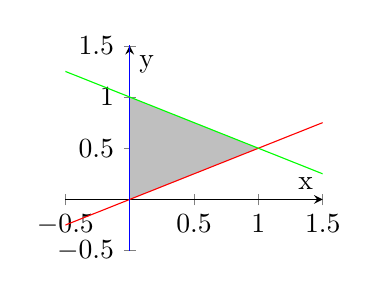
\begin{tikzpicture}
            \begin{axis}[width=0.4\textwidth, axis lines=middle, xlabel=x, ylabel=y, xmin=-.5, ymin=-.5, ymax=1.5, xmax=1.5]
                \addplot[fill=lightgray,draw=none] coordinates{(0, 0) (0, 1) (1, 0.5)};
                \addplot[color=red]{0.5*x};
                \addplot[color=blue] table[row sep = crcr]{0 -11 \\ 0 11 \\};
                \addplot[color=green]{1-0.5*x};
            \end{axis}
        \end{tikzpicture}
    \end{figure}
    The shaded region (we'll call it \( D \)) is what we want to integrate over. This region can be paramaterized:
    \[ D = \left\{ (x,y)\quad |\quad 0\leq x\leq 1,\quad \frac{1}{2}x\leq y\leq 1-\frac{1}{2}x\right\}\]
    Then, we can set up and compute our double integral,
    \begin{align*}
        V &= \iint\limits_D \bqty{2-x-2y}\dd A = \int_0^1\int_{\frac{1}{2}x}^{1-\frac{1}{2}x}\bqty{2-x-2y}\dd y\dd x \\
        &= \int_0^1 \bqty{2y-xy-y^2}_{y=x/2}^{y=1-x/2}\dd x \\
        &= \int_0^1\bqty{2\pqty{1-\frac{1}{2}x}-x\pqty{1-\frac{1}{2}x}-\pqty{1-\frac{1}{2}x}^2 - 2\pqty{\frac{x}{2}}+x\pqty{\frac{x}{2}}-\pqty{\frac{x}{2}}^2}\dd x \\
        &= \int_0^1 [x^2-2x+1]\dd x = \frac{x^3}{3}-x^2+x\biggr|_0^1 = \boxed{\frac{1}3} 
    \end{align*}
\end{example}
\subsubsection{Properties of Double Integrals}
First, let \( f: \RR^n\to\RR \) and \( g: \RR^n\to\RR \) both be integrable on a region \( D\subseteq \RR^n \), and let \( c\in\RR \) be constant. Then, 
\begin{align}
    \int\limits_D [f+g]\dd^n A &= \int\limits_D f\dd^n A + \int\limits_Dg\dd^n A \\
    \int\limits_D cf\dd^n A &= c\int\limits_D f\dd^n A
\end{align}
If \( f \geq g \) on \( D \), then
\begin{align}
    \int\limits_D f\dd^n A \geq \int\limits_D g\dd^n A
\end{align}
If \( D \) can be expressed as the union of several disjoint regions (except perhaps on their boundaries) \( D_1,D_2,\dots,D_n \)--that is, \( D = \bigcup_{i=1}^{n}D_i \) where \( \bigcap_{i=1}^n D_i\setminus \partial D_i = \varnothing \),
\[ \int\limits_D f\dd^n A = \sum_{i=1}^n \int\limits_{D_i}f\dd^n A\]
The next property states that if we integrate the constant function \( f = 1 \), we get the area (or volume, or etc. in higher dimensions) of \( D \).
\[ \int\limits_D \dd^n A = A(D)\]
These properties can be combined to tell us,
\begin{theorem} \label{area}
    If \( L, U\in\RR \), and \( f: \RR^n\mapsto \RR \) is integrable on a region \( D\subseteq \RR^n \), with \( L \leq f(\vec x) \leq U \) for all \( x\in D \),
    \[ LA(D) \leq \int\limits_Df\dd^nA \leq UA(D)\] 
    Where \( A(D) \) is the area (or \( n \)-dimensional equivalent) of \( D \).
\end{theorem}
\begin{example}
    Estimate the integral \( \iint\limits_D e^{\sin x\cos y}\dd A \) where \( D \) is the disk centered on the origin with radius \( 2 \). \par\bf{Solution: }First, recognize that the area of \( D \) is given by \( \pi r^2 = 4\pi \), and that \( -1 \leq \sin x\cos y \leq 1 \), so \( \frac{1}{e} \leq e^{\sin x\cos y} \leq e \) on \( D \). Therefore, 
    \[ 4\pi e^{-1} \leq \iint\limits_D e^{\sin x\cos y}\dd A \leq 4\pi e\] 
    Or,
    \[ 4.623 \leq \iint\limits_D e^{\sin x\cos y}\dd A \leq 34.159\]
\end{example}
\subsection{Double Integrals in Polar Coordinates}
Some regions are much easier to describe and integrate over with polar coordinates. \par 
Consider a region \( R = \{(r, \theta), a\leq r\leq b, \alpha \leq \theta \leq \beta\} \). This is called a \it{polar rectangle}. To define integration over this region, divide the interval \( [a,b] \) into \( m \) equal sub-intervals where \( \Delta r = (b-a)/m \). Similarly, divide the interval \( [\alpha, \beta] \) into \( n \) equal sub-intervals where \( \Delta \theta = (\beta - \alpha)/n \). Then, each infinitesimal segment of area \( A_{ij} \) is defined by the rays \( r = r_i \) and \( r = r_{i+1} = r_i + \Delta r \), along with \( \theta = \theta_j \) and \( \theta = \theta_{j+1} = \theta_j + \Delta \theta \).\par
Recall that the area of a sector of a circle with radius \( \ell \) and central angle \( \phi \) is \( \frac{1}{2}\ell^2\phi \). Applying this to our scenario, each infinitesimal section of area is equivalent to the area of a sector formed by \( \theta \in [\theta_j, \theta_{j+1}] \) and \( r = r_{i+1} \) \it{minus} the area of the sector formed by \( \theta\in[\theta_j, \theta_{j+1}] \) and \( r = r_i \). That is,
\begin{align*}
    A_{ij} &= \frac{1}{2}r_{i+1}^2(\theta_{j+1}-\theta_j) - \frac{1}{2}r_i^2(\theta_{j+1}-\theta_j) \\
    &= \frac{1}{2}(\theta_{j+1}-\theta_j)(r_{i+1}^2-r_i^2) \\
    &= \frac{1}{2}\Delta \theta (r_{i+1}-r_i)(r_{i+1}+r_i)
\end{align*}
Noticing that the radius of the center of the sector is \( r_i^* = \frac{1}{2}(r_{i+1}+r_i) \), we arrive at
\begin{align*}
    A_{ij} &= r_i^*\Delta r\Delta \theta
\end{align*}
So the Riemann sum describing the area can be expressed as
\begin{align*}
    \sum_{i=1}^m\sum_{j=1}^n r_i^*\Delta r \Delta \theta
\end{align*}
Or, if we have a function \( f(x, y) \), the double integral \( \iint\limits_Rf\dd A \) is,
\begin{align*}
    \sum_{i=1}^m\sum_{j=1}^nf(r_i^*\cos\theta_j^*, r_i^*\sin\theta_j^*) r_i^*\Delta r \Delta \theta
\end{align*}
Therefore, we have
\[ \iint\limits_R f(x, y)\dd A = \int_{\alpha}^{\beta}\int_{a}^bf(r\cos\theta, r\sin\theta)r\dd r\dd \theta \]
This can be thought of as integrating \( f \) over infinitely many polar rectangles, each one having area \( \dd A = r\dd r\dd \theta \) (because \( r\dd \theta \) is the arc length of the polar regions, which becomes closer to being straight and forming a rectangle with the side \( \dd r \) as \( \dd \theta \to 0 \)).
\begin{example}
    Evaluate \( \iint\limits_R(3x+4y^2)\dd A \), where \( R \) is the region bounded by \( x^2+y^2=1 \), \( x^2+y^2=4 \), and the line \( y=0 \). \par\bf{Solution}:
    \( R \) can be expressed as \( R = \{ (r,\theta)|1\leq r\leq 2, 0\leq \theta\leq \pi\} \). Therefore,
    \begin{align*}
        \iint\limits_R (3x+4y^2)\dd A &= \int_0^\pi\int_1^2(3r\cos\theta + 4r^2\sin^2\theta)r\dd r\dd \theta \\
        &= \int_0^\pi\int_1^2(3r^2\cos\theta + 4r^3\sin^2\theta)\dd r\dd \theta \\
        &= \int_0^\pi\pqty{r^3\cos\theta+r^4\sin^2\theta\biggr|_{r=1}^{r=2}}\dd \theta \\
        &= \int_0^\pi (8\cos\theta + 16\sin^2\theta - \cos\theta - \sin^2\theta)\dd \theta \\
        &= \int_0^\pi \pqty{7\cos\theta + \frac{15}{2}(1-\cos(2\theta)}\dd \theta \\
        &= 7\sin\theta + \frac{15}{2}\theta -\frac{15}{4}\sin(2\theta)\biggr|_{\theta=0}^{\theta=\pi} = \boxed{\frac{15\pi}{4}}
    \end{align*}
\end{example}
The power reduction trig identities will be very helpful for these types of integrals, and are worth remembering.
\[ \sin^2x = \frac{1}{2}(1-\cos 2x), \quad \cos^2x = \frac{1}{2}(1+\cos 2x) \]
\begin{example}
    Find the volume of the solid bounded by the plane \( z=0 \) and the paraboloid \( z=1-x^2-y^2 \). \par\bf{Solution}: 
    First, we can find the intersection of the paraboloid with the plane \( z=0 \):
    \[ 0 = 1-x^2-y^2 \quad\implies\quad x^2+y^2=1\]
    So the region is the unit circle on the \( xy \)-plane, or \( R = \{(r, \theta)|0\leq r\leq 1, 0\leq\theta\leq 2\pi\} \). So the volume is given by
    \begin{align*}
        V &= \int_0^{2\pi}\int_0^1(1-x^2-y^2)r\dd r\dd \theta \\
        &= \int_0^{2\pi}\int_0^1 (1-r^2)r\dd r\dd\theta \\
        &= \int_0^{2\pi}\int_0^1 r-r^3\dd r\dd \theta \\
        &= \int_0^{2\pi}\bqty{\frac{1}{2}r^2-\frac{1}{4}r^4}_{r=0}^{r=1}\dd \theta \\
        &= \int_0^{2\pi}\frac{1}{4}\dd \theta = \boxed{\frac{\pi}{2}}
    \end{align*}
    This is a good example of a case where polar is a much easier method of integration. If we were to integrate in rectangular, we would have
    \[ V = \int_{-1}^1\int_{-\sqrt{1-x^2}}^{\sqrt{1-x^2}}[1-x^2-y^2]\dd y\dd x \]
    Which would require some very advanced integration techniques, since you would have to find 
    \[ \int \sqrt{1-x^2}\dd x, \quad \int x^2\sqrt{1-x^2}\dd x,\quad\text{and}\quad \int(1-x^2)^{3/2}\dd x \]
\end{example}
Similar to double integrals over general rectangular regions, if we have a polar region that can be expressed as 
\[ R = \{(r, \theta)| \alpha\leq \theta \leq \beta, h_1(\theta)\leq r\leq h_2(\theta)\}\]
then \( \iint\limits_Rf(x,y)\dd A \) can be written as 
\[ \iint\limits_Rf(x,y)\dd A = \int_\alpha^\beta\int_{h_1(\theta)}^{h_2(\theta)} f(r\cos\theta, r\sin\theta)r\dd r \dd \theta\]
Choosing \( f(x,y)=1 \), we can get the area of a polar region:
\[ A(R) = \iint\limits_R\dd A =\int_{\alpha}^{\beta}\int_{h_1(\theta)}^{h_2(\theta)}r\dd r\dd \theta = \int_{\alpha}^{\beta}\frac{1}{2}(h_2(\theta)^2-h_1(\theta)^2)\dd \theta\]
Which you may recognize as the formula for the area between two polar graphs from Calculus 1. 
\begin{example}
    Use a double integral to find the area enclosed by one loop of the four-leaved rose \( r=\cos(2\theta) \). \par\bf{Solution: }First, we want to find the bounds, which will occur at the \( \theta \) values where \( \cos(2\theta) = 0 \). The two that we are concerned with are \( \theta = -\pi/4 \) and \( \theta = \pi/4 \). Therefore, our double integral is
    \begin{align*}
        A &= \int_{-\pi/4}^{\pi/4}\int_0^{\cos(2\theta)}r\dd r\dd \theta \\
        &= \int_{-\pi/4}^{\pi/4} \frac{1}{2}\cos^2(2\theta)\dd \theta \\
        &= \int_{-\pi/4}^{\pi/4} \frac{1}{4}(1+\cos(4\theta))\dd\theta \\
        &= \frac{\theta}{4} + \frac{1}{16}\sin(4\theta)\biggr|_{-\pi/4}^{\pi/4} = \boxed{\frac{\pi}{8}}
    \end{align*}
\end{example}
\begin{example}
    Find the volume of the solid that lies under the paraboloid \( z=x^2+y^2 \) above the \( xy \)-plane, and inside the cylinder \( x^2+y^2=2x \). \par\bf{Solution: }First, we want to rewrite our bounds in a way that can be expressed in polar.
    \begin{align*}
        0 &= x^2-2x+y^2 \\
          &= (x-1)^2 + y^2 - 1
    \end{align*}
    Or \( (x-1)^2+y^2=1 \). This is a circle of radius \( 1 \) centered at the point \( (1, 0) \). Now, to express this in polar, we will want to perform a coordinate shift. Note that if we let \( u = x-1 \), then our circle equation becomes \( u^2+y^2=1 \), which is centered at our "new origin." Our paraboloid equation then becomes \( z=(u+1)^2+y^2 \), which we can now integrate.
    \begin{align*}
        \iint\limits_R (x^2+y^2)r\dd r\dd \theta &= \int_0^{2\pi}\int_0^1[(u+1)^2+y^2]r\dd r\dd \theta \\
        &= \int_0^{2\pi}\int_0^1 r(r\cos\theta + 1)^2 + r^3\sin^2\theta \dd r\dd \theta \\
        &= \int_0^{2\pi}\int_0^1 r^3\cos^2\theta + 2r^2\cos\theta + r + r^3\sin^2\theta \dd r\dd \theta \\
        &= \int_0^{2\pi}\int_0^1 r^3(\cos^2\theta+\sin^2\theta) + 2r^2\cos\theta + r \dd r\dd \theta \\
        &= \int_0^{2\pi}\int_0^1 r^3+2r^2\cos\theta + r\dd r\dd \theta \\
        &= \int_0^{2\pi}\bqty{\frac{1}{4}r^4+\frac{2}{3}r^3\cos\theta+\frac{1}{2}r^2\biggr|_{r=0}^{r=1}} \\
        &= \int_0^{2\pi} \frac{3}{4}+\frac{2}{3}\cos\theta = \frac{3}{2}\theta + \frac{2}{3}\sin\theta\biggr|_0^{2\pi} = \boxed{\frac{3\pi}{2}}
    \end{align*}
\end{example}
\subsection{Applications of Double Integrals}
We've already explored one application of double integrals in computing volume. Now, we will look at some other ones such as computing mass, electric charge, center of mass, moments, and probabilities.
\subsubsection{Density and Mass}
If we have an object that occupies a region \( D \) in the \( xy \)-plane, and has a variable area density function \( \rho_A(x,y) \) that is continuous on \( D \), then we can write the mass of the object as 
\[ m = \lim_{k,l\to\infty}\sum_{i=1}^k\sum_{j=1}^l \rho_A(x_i^*, y_j^*)\Delta A = \iint\limits_D \rho_A(x,y)\dd A \]
Another similar application is using charge densities to find the total charge in a charge distribution. If the charge distribution is given by an integrable function \( \sigma(x,y) \), then the total charge is given by
\[ Q = \iint\limits_D \sigma(x,y)\dd A \]
\begin{example}
    Charge is distributed over a triangular region \( D \) enclosed by \( y=1 \), \( x=1 \), and \( y=1-x \), where \( x \) and \( y \) are measured in meters. The charge density at a point \( (x,y) \) on \( D \) is given by \( \sigma(x,y)=xy \), where \( \sigma \) is measured in coulombs per square meter. Find the total charge on \( D \). \par\bf{Solution}: Our double integral can be written as
    \begin{align*}
        \iint\limits_D\sigma(x,y)\dd A &= \int_0^1\int_{1-x}^{1}xy\dd y\dd x \\
        &= \int_0^1 \frac{1}{2}xy^2\biggr|_{y=1-x}^{y=1}\dd x \\
        &= \frac{1}{2}\int_0^1x - x(1-x)^2 \dd x \\
        &= \frac{1}{2}\int_0^1 x - x^3 + 2x^2 - x\dd x \\
        &= \frac{1}{2}\bqty{\frac{2}{3}x^3-\frac{1}{4}x^4\biggr|_{0}^1} = \boxed{\frac{5}{24}}
    \end{align*}
\end{example}
\subsubsection{Moments and Center of Mass}
Suppose we have a lamina occupying a region \( D \) with a density function \( \rho_A(x,y) \). Then, the \bf{moment} of the lamina about the x-axis is
\[ M_x = \iint\limits_D y\rho(x,y)\dd A\]
and the moment of the lamina about the y-axis is
\[ M_y = \iint\limits_D x\rho(x,y)\dd A \]
We define the center of mass \( \< \overline{x},\overline{y} \> \) of the lamina so that if the total mass is \( m \), then \( m\overline{x}=M_x \) and \( m\overline{y}=M_y \). That is,
\begin{align*}
    \overline{x} &= \frac{M_x}{m} = \frac{\iint\limits_D y\rho(x,y)\dd A}{\iint\limits_D \rho(x,y)\dd A} \\
    \overline{y} &= \frac{M_y}{m} = \frac{\iint\limits_D x\rho(x,y)\dd A}{\iint\limits_D \rho(x,y)\dd A}
\end{align*}
\begin{example}
    Find the mass and center of mass of a triangular lamina with vertices \( (0,0) \), \( (1,0) \), and \( (0, 2) \) if the density function is \( \rho(x,y) = 1+3x+y \).\par\bf{Solution: }First, let's draw a picture. \par
    \begin{figure}[h!]
        \centering
        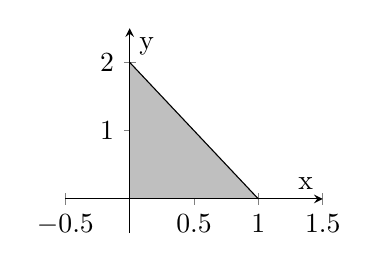
\begin{tikzpicture}
            \begin{axis}[width=0.4\textwidth, axis lines=middle, xlabel=x, ylabel=y, xmin=-.5, ymin=-.5, ymax=2.5, xmax=1.5]
                \addplot[fill=lightgray,draw=none] coordinates{(0, 0) (1, 0) (0, 2)};
                \addplot[color=black] table[row sep = crcr]{0 0 \\ 0 2 \\};
                \addplot[color=black] table[row sep = crcr]{0 0 \\ 1 0 \\};
                \addplot[color=black] table[row sep = crcr]{1 0 \\ 0 2 \\};
            \end{axis}
        \end{tikzpicture}
    \end{figure}
    Let's call the shaded region \( D \). We can write \( D \) as 
    \[ D = \{(x,y)|0\leq x\leq 1, 0\leq y \leq 2-2x\}\]
    So the mass of the lamina is
    \begin{align*}
        m = \iint\limits_D \rho(x,y)\dd A &= \int_0^1\int_0^{2-2x}[1+3x+y]\dd y\dd x \\
        &= \int_0^1 \bqty{y+3xy+\frac{1}{2}y^2}_{y=0}^{y=2-2x}\dd x \\
        &= \int_0^1 (2-2x)+3x(2-2x)+\frac{1}{2}(2-2x)^2\dd x \\
        &= \int_0^1 4-4x^2\dd x = 4\bqty{x-\frac{1}{3}x^3}_0^1 = \boxed{\frac{8}{3}}
    \end{align*}
\end{example}
Then, center of mass in the \( x \) direction:
\begin{align*}
    \overline x = \frac{1}{m}\iint\limits_D x\rho(x,y)\dd A &= \frac{3}{8}\int_0^1\int_0^{2-2x}[x+3x^2+xy]\dd y\dd x \\
    &= \frac{3}{8}\int_0^1\bqty{xy+3x^2y+\frac{1}{2}xy^2}_{y=0}^{y=2-2x}\dd x \\
    &= \frac{3}{8}\int_0^1\bqty{2x-2x^2 + 6x^2-6x^3 + 2x-4x^2+2x^3}\dd x \\
    &= \frac{3}{8}\int_0^1\bqty{-4x^3+4x}\dd x = \frac{3}{2}\int_0^1 (x-x^3)\dd x \\
    &= \frac{3}{2}\bqty{\frac{1}{2}x^2-\frac{1}{4}x^3}_0^1 = \boxed{\frac{3}{8}}
\end{align*}
And in the \( y \) direction:
\begin{align*}
    \overline y = \frac{1}{m}\iint\limits_D y\rho(x,y)\dd A &= \frac{3}{8}\int_0^1\int_0^{2-2x}[y+3xy+y^2]\dd y\dd x \\
    &= \frac{3}{8}\int_0^1 \bqty{\frac{1}{2}y^2+\frac{3}{2}xy^2+\frac{1}{3}y^3}_0^{2-2x}\dd x \\
    &= \frac{3}{8}\int_0^1 \bqty{\frac{1}{2}(2-2x)^2+\frac{3}{2}x(2-2x)^2+\frac{1}{3}(2-2x)^3}\dd x \\
    &= \frac{3}{8}\int_0^1 \bqty{2x^2-4x+2+6x^3-12x^2+6x-\frac{8}{3}x^3+8x^2-8x+\frac{8}{3}}\dd x \\
    &= \frac{1}{4}\int_0^1 \bqty{5x^3-3x^2-9x+7}\dd x = \frac{1}{4}\bqty{\frac{5}{4}x^4-x^3-\frac{9}{2}x^2+7x}_0^1 \\
    &= \frac{1}{4}\bqty{\frac{5}{4}-\frac{4}{4}-\frac{18}{4}+\frac{28}{4}} = \boxed{\frac{11}{16}}
\end{align*}
\begin{example}
    The density at a point on a semicircular lamina of radius \( a \) is proportional to the distance from the center of the circle. Find the center of mass of the lamina. \par\bf{Solution: }First, write out the density function: 
    \[ \rho = k\sqrt{x^2+y^2} = kr \]
    Then, integrate over the circle in polar coordinates:
    \begin{align*}
        m = \iint\limits_D \rho\dd A &= \int_0^\pi\int_0^ar\rho\dd r\dd \theta \\
        &= \int_0^\pi\int_0^a kr^2\dd r\dd \theta \\
        &= \int_0^\pi \frac{1}{3}ka^3\dd \theta = \frac{ka^3\pi}{3}
    \end{align*}
    Because of the symmetry of the lamina, we can reason that the center of mass in the \( x \) direction will be on the \( y \) axis (but we'll integrate it anyway just to verify)
    \begin{align*}
        \overline{x} = \frac{1}{m}\iint\limits_D x\rho \dd A &= \frac{3}{ka^3\pi}\int_0^\pi\int_0^a kr^3\cos\theta \dd r\dd \theta \\
        &= \frac{3}{ka^3\pi}\int_0^\pi \frac{1}{3}kr^3\cos\theta\dd \theta = \frac{3}{ka^3\pi}\bqty{\frac{1}{4}ka^4\sin\theta}_0^\pi = 0
    \end{align*}
    and
    \begin{align*}
        \overline{y} = \frac{1}{m}\iint\limits_D y\rho\dd A &= \frac{3}{ka^3\pi}\int_0^\pi\int_0^a kr^3\sin\theta \dd r\dd \theta \\
        &= \frac{3}{ka^3\pi}\int_0^\pi \frac{1}{4}ka^3\sin\theta\dd \theta \\
        &= -\frac{3}{ka^3\pi}\bqty{\frac{1}{4}ka^4\cos\theta}_0^\pi = \frac{3a}{2\pi}
    \end{align*}
\end{example}
\subsubsection{Moments of Inertia}
The moment of inertia (also called the second moment) of a particle with mass \( m \) about an axis is defined to be \( mr^2 \), where \( r \) is the distance between the particle and the axis. We can extend this definition to two-dimensional mass distributions. \par
Consider a lamina with density function \( \rho(x,y) \) that occupies a region \( D \). We can divide \( D \) into \( m \) sub-rectangles in the \( x \) direction and \( n \) sub-rectangles in the \( y \) direction, and let \( m \) and \( n \) tend to infinity. Then, we can choose two sample points \( x_i^*\in [x_i, x_{i+1}] \) and \( y_j^*\in [y_j, y_{j+1}] \) for each sub-rectangle \( (i, j) \). The distance between the \( x \) axis and the sample point is then \( y_j^* \). Then, we sum up the contributions to the overall inertia from each sub-rectangle.
\[ I_x = \lim_{m,n\to\infty}\sum_{i=1}^m\sum_{j=1}^n (y_j^*)^2\rho(x_i^*, y_j^*)\Delta A = \iint\limits_D y^2\rho(x,y)\dd A \]
The moment of inertia about the $y$ axis is found similarly, 
\[ I_x = \lim_{m,n\to\infty}\sum_{i=1}^m\sum_{j=1}^n (x_i^*)^2\rho(x_i^*, y_j^*)\Delta A = \iint\limits_D x^2\rho(x,y)\dd A \]
We can also consider a moment of inertia about the origin (this can be thought of as an object rotating about what would be the $z$ axis in three-dimensional space). We again split $D$ into sub-rectangles, but now the distance to the sample point is given by \( \sqrt{(x_i^*)^2+(y_j^*)^2} \), so we find
\[ I_0 =  \lim_{m,n\to\infty}\sum_{i=1}^m\sum_{j=1}^n ((x_i^*)^2+(y_j^*))\rho(x_i^*, y_j^*) = \iint\limits_D (x^2+y^2)\rho(x,y)\dd A \]
Note that the equivalency $I_0 = I_x + I_y$ holds because we can split up the integral as such:
\[ \iint\limits_D (x^2+y^2)\rho(x,y)\dd A = \iint\limits_D y^2\rho(x,y)\dd A + \iint\limits_D x^2\rho(x,y)\dd A = I_x + I_y \]
\begin{example}
    Find the moments of inertia \(I_x\), \(I_y\), and \(I_0\) of a homogeneous disk \(D\) with density \(\rho(x,y) = \rho\), center \((0,0)\) and radius \(a\). \par
    \bf{Solution: }Let's first find \(I_0\).
    \[ I_0 = \iint\limits_D (x^2+y^2)\rho(x,y)\dd A = \iint\limits_D (x^2+y^2)\rho\dd A \]
    Note that \(D\) can be written as \( \{(r,\theta)| 0\leq\theta\leq2\pi, 0\leq r\leq a\} \), so we can rewrite
    \begin{align*}
        I_0 = \iint\limits_D(x^2+y^2)\rho \dd A &= \int_0^{2\pi}\int_0^ar^3\rho \dd r\dd \theta \\
        &= \frac{\rho a^4}{4}\int_0^{2\pi}\dd \theta = \frac{\rho\pi a^4}{2}
    \end{align*}
    Because of the symmetry of the problem, we can see that $I_x = I_y = \frac{1}{2}I_0$. Therefore,
    \[ \boxed{I_0 = \frac{\rho\pi a^4}{2}, \quad I_x = I_y = \frac{\rho\pi a^4}{4}} \]
    If we notice that the mass of the disk will be \(\rho\pi a^2\) (density $\times$ area), we can rewrite \( I_0\) as \( I_0 = \frac{1}{2}ma^2 \), which you may recognize as the moment of inertia of a disk about its axle from physics. This is an alternate derivation for it.
\end{example}
We can also define a quantity called the \bf{radius of gyration} about an axis. We define it as the number \( R \) such that 
\[ mR^2 = I \]
where \( m \) is the mass of the lamina and \( I \) is the moment of inertia about the given axis. \par 
The radius of gyration can be thought of as the point where, if we were to concentrate the entire mass of the lamina there, would not affect the moment of inertia. \par 
We can define the radius of gyration \( \overline{\overline{y}} \) with respect to the $x$-axis and the radius of gyration \( \overline{\overline{x}} \) with respect to the $y$-axis as 
\[ m\overline{\overline{y}}^2 = I_x, \quad m\overline{\overline{x}}^2 = I_y\]
We can also define the radius of gyration \( \overline{\overline{r}} \) with respect to the origin as the number $\overline{\overline{r}}$ such that
\[ m\overline{\overline{r}}^2 = I_0 \]
\begin{example}
    Find the radius of gyration about the $x$-axis of the disk in the previous example.\par
    \bf{Solution: }Recall that the moment of inertia about the $x$ axis is \( I_x = (1/4)\rho \pi a^4 \) and the mass of the disk is \( \rho \pi a^2\). So we can find \( \overline{\overline{y}} \) with
    \[ \overline{\overline{y}} = \sqrt{\frac{I_x}{m}} = \sqrt{\frac{\rho \pi a^4}{4\rho \pi a^2}} = \frac{a}{2}\]
\end{example}
\subsubsection{Probability}
Let $f: \RR\to\RR$ be a probability density function of a continuous random variable $X$. This means that $f$ must satisfy two criteria:
\begin{enumerate}
    \item \(\int_{-\infty}^\infty f(x)\dd x = 1\).
    \item the probability that \(X\in[a,b]\) is found with \(P(a\leq X\leq b) = \int_a^bf(x)\dd x\).
\end{enumerate}
One common probability density function is the normal distribution, defined with
\[ f(x) = \frac{1}{\sigma\sqrt{2\pi}}e^{-\frac{1}{2}\pqty{\frac{x-\mu}{\sigma}}^2}\]
Where \(\sigma\) is the mean of the dataset and \( \mu\) is the standard deviation. It is left as an exercise to reader to verify that \( \int_{-\infty}^\infty f(x)\dd x = 1\) (this will actually require some methods of multivariable calculus, despite it being a single integral). \par
Now, let $f: \RR^2\mapsto \RR$ be a probability density function of a pair of continuous random variables \((X,Y)\). This is known as a \bf{joint density function}, and satisfies similar criteria to single-variable probability density functions.
\begin{enumerate}
    \item \(\iint\limits_{\RR^2} f(x,y)\dd A = 1\).
    \item The probability that \((X,Y)\in D\) for some \(D\subset \RR^2\) is found with \(P((X,Y)\in D) = \iint\limits_D f(x,y)\dd A\).
\end{enumerate}
Similarly, we can define a joint density function for a set of $n$ continuous random variables \( X_1, X_2, \dots, X_n \) as a function \(f: \RR^n\to\RR\) that satisfies 
\begin{enumerate}
    \item \(\int\limits_{\RR^n} f(\vec x)\dd^n\vec x = 1\).
    \item The probability that \((X_1, X_2, \dots, X_n)\in D\) for some \(D\subset \RR^n\) is found with \(P((X_1, X_2, \dots, X_n)\in D) = \int\limits_D f(\vec x)\dd^n\vec x\).
\end{enumerate}
\begin{example}
    If the joint density function for \(X\) and \(Y\) is given by 
    \[ f(x,y) = \begin{cases}
        C(x+2y) & x\in [0, 10], y\in[0, 10] \\
        0 & \text{otherwise}
    \end{cases}\]
    find the value of the constant $C$. Then, find $P(X\leq 7, Y\geq 2)$.\par
    \bf{Solution: }First, let's find $C$. Remember that $f$ must satisfy $\iint\limits_{\RR^2}f(x,y)\dd A = 1$. So,
    \begin{align*}
        \iint\limits_{\RR^2}f(x,y)\dd A = \int_{-\infty}^\infty\int_{-\infty}^{\infty}f(x,y)\dd y\dd x
    \end{align*}
    But because $f(x,y) = 0$ for all $(x,y)$ not in the square of sidelength $10$ centered at the origin, we can rewrite
    \begin{align*}
        \int_{-\infty}^\infty\int_{-\infty}^{\infty}f(x,y)\dd y\dd x &= \int_{0}^{10}\int_{0}^{10}C(x+2y)\dd y\dd x \\
        &= C\int_{0}^{10}\int_{0}^{10}(x+2y)\dd y\dd x \\
        &= C \int_0^{10} \bqty{xy+y^2}_{y=0}^{y=10}\dd x\\
        &= C\int_0^{10} [10x+100]dx \\
        &= C\bqty{5x^2+100x}_0^{10} = 1500C
    \end{align*}
    So because $1500C=1$, $C=\frac{1}{1500}$.\par
    Now, finding $P(X\leq 7, Y\geq 2)$, we can write it as an iterated integral
    \begin{align*}
        P(X\leq 7, Y\geq 2) &= \int_{-\infty}^{7}\int_{2}^\infty f(x,y)\dd y\dd x
    \end{align*}
    Again, since $f(x,y) = 0$ for all $(x,y)$ not in the square of sidelength $10$ centered at the origin, we can rewrite to
    \begin{align*}
        P(X\leq 7, Y\geq 2) &= \int_{0}^{7}\int_{2}^{10} C(x+2y)\dd y\dd x \\
        &= C\int_0^7 \bqty{xy+y^2}_{y=2}^{y=10}\dd x\\
        &= C\int_0^7 8x+96\dd x = C\bqty{4x^2+96x}_0^7 \\
        &= 868C = \frac{868}{1500} \approx 0.579
    \end{align*}
\end{example}
In the above examples, the probaility for a given value of $Y$ depended on the value of $X$. That is not always the case. When it isn't, we call $X$ and $Y$ \bf{independent random variables}. Then, their joint density function is simply the product of their individual density functions.
\[ f(x,y) = f_1(x)f_2(y) \]
It can be shown that if $f_1$ and $f_2$ satisfy the criteria for a probability density function, then $f$ will satisfy the criteria for a joint probability density.
\begin{align*}
    \iint\limits_{\RR^2} f(x,y)\dd A &= \int_{-\infty}^{\infty}\int_{-\infty}^{\infty}f_1(x)f_2(y)\dd y\dd x \\
    &= \bqty{\int_{\infty}^\infty f_1(x)\dd x}\bqty{\int_{\infty}^\infty f_2(y)\dd y} \\
    &= 1\cdot 1 = 1
\end{align*}
Consider the exponential density function
\[ f(t) = \begin{cases}
    0 & t < 0 \\
    \mu^{-1}e^{-t/\mu} & t\geq 0
\end{cases}. \]
This can be used to model the probabilities of waiting times, where $\mu$ is the mean waiting time.
\begin{example}
The manager of a movie theater determines that the average time moviegoers
wait in line to buy a ticket for this week's film is $10$ minutes and the average time they wait to buy popcorn is $5$ minutes. Assuming that the waiting times are independent, find the probability that a moviegoer waits a total of less than $20$ minutes before taking their seat using the exponential density model. \par
\bf{Solution: }The density functions for the movie ticket waiting time ($x$) and popcorn waiting time ($y$) respectively are
\[ f_1(x) = \begin{cases}
    0 & x < 0 \\
    e^{-x/10}/10 & x > 0
\end{cases}\quad\text{and}\quad f_2(y)=\begin{cases}
    0 & y < 0 \\
    e^{-y/5}/5 & y > 0
\end{cases} \]
So the joint density function is
\[ f(x,y) = \begin{cases}
    \bqty{\frac{e^{-x/10}}{10}}\bqty{\frac{e^{-y/5}}{5}} & x > 0, y > 0 \\
    0 & \text{otherwise}
\end{cases} \]
This simplifies to
\[ f(x,y) = \begin{cases}
    \frac{1}{50}e^{-x/10}e^{-y/5} & x > 0, y > 0 \\
    0 & \text{otherwise}
\end{cases} \]
If the total time the moviegoer waits is less than $20$ minutes, then we must have $x+y < 20$. Clearly, $x$ and $y$ must be positive because it is nonsensical to have negative waiting times. Therefore, the valid pairs $(x,y)$ are described by the region
\[ R = \{(x,y)|0\leq x < 20, 0\leq y< 20-x \} \]
So the probability that a moviegoer waits less than 20 minutes is given by
\begin{align*}
    P((x,y)\in R) = \iint\limits_R f(x,y)\dd A = \int_0^{20}\int_0^{20-x}f(x,y)\dd y\dd x
\end{align*}
Because we never have $x$ or $y$ negative, we can rewrite as
\begin{align*}
    P((x,y)\in R) &= \int_0^{20}\int_0^{20-x} \frac{1}{50}e^{-x/10}e^{-y/5}\dd y\dd x \\
    &= -\frac{1}{10}\int_0^{20}\bqty{e^{-x/10}e^{-y/5}}_{y=0}^{y=20-x}\dd x \\
    &= -\frac{1}{10}\int_0^{20}e^{-x/10}\pqty{e^{-(20-x)/5}-1}\dd x \\
    &= -\frac{1}{10}\int_0^{20}e^{-4 + x /5 - x/10}-e^{-x/10}\dd x \\
    &=-\frac{1}{10}\int_0^{20}e^{-4}e^{x/10}-e^{-x/10}\dd x \\
    &=-\pqty{e^{-4}e^{x/10}+e^{-x/10}}\biggr|_0^{20} = 1+e^{-4}-2e^{-2} \approx 0.748
\end{align*}
\end{example}
\subsubsection{Expected Value}
The expected values $(\mu_1, \mu_2)$ of a probability function $f(x,y)$ are the first moments of $f$ with respect to $x$ and $y$ respectively. That is,
\begin{align*}
    \mu_1 = \iint\limits_{\RR^2}xf(x,y)\dd A, \qquad \mu_2 = \iint\limits_{\RR^2}yf(x,y)\dd A 
\end{align*}
We can justify this by imagining the probability density function as describing a sort of ``probability mass." The total mass is given by \( \iint_{\RR^2}f(x,y)\dd A \), which we know to be $1$ from the definition of a probability density function. Then, the expected value is analogous to the center of mass, which is qual to the moment divided by the mass. However, since the mass is $1$, it is just equal to the moment.
\subsection{Surface Area}
Another application of double integrals is computing the area of a surface. \par
Consider a graph $z=f(x,y)$ of two variables that is differentiable along a region $D\subset \RR^2$. Let $U$ be the surface represented by $z=f(x,y)$ where $(x,y)\in D$. If we split $D$ into $m$ sub-rectangles in the $x$ direction and $n$ sub-rectangles in the $y$ direction and choose a sample point $x_i^*\in[x_i,x_{i+1}]$, $y_j^*\in[y_j, y_{j+1}]$, we can use the area of the tangent plane of $f$ at $(x_i^*, y_j^*)$ along the sub-rectangle to approximate the area of the function. \par
The tangent vectors to $f$ in the $x$ and $y$ direction are given by 
\[ \vec t_x = \< \Delta x, 0, f_x(x_i^*, y_j^*)\>\quad\text{and}\quad \vec t_y = \< 0, \Delta y, f_y(x_i^*, y_j^*) \> \]
and the area of the parallellogram formed by $\vec t_x$ and $\vec t_y$ is given by 
\begin{align*}
    \dd S = \norm{\vec t_x\times \vec t_y}  &= \begin{vmatrix}
        \ihat & \jhat & \khat \\
        \Delta x & 0 & \Delta xf_x(x_i^*, y_j^*) \\
        0 & \Delta y & \Delta yf_y(x_i^*, y_j^*)
    \end{vmatrix} \\
    &= \norm{\< -\Delta y\Delta xf_x(x_i^*, y_j^*), -\Delta y\Delta xf_y(x_i^*, y_j^*), \Delta x\Delta y \>} \\
    &= \sqrt{\bqty{-\Delta y \Delta xf_x(x_i^*, y_j^*)}^2 + \bqty{-\Delta y\Delta xf_y(x_i^*, y_j^*)}^2 + \bqty{\Delta x + \Delta y}^2} \\
    &= \sqrt{\bqty{f_x(x_i^*, y_j^*)}^2 + \bqty{f_y(x_i^*, y_j^*)}^2 + 1}\, \Delta y\Delta x \\
    &= \sqrt{\bqty{f_x(x_i^*, y_j^*)}^2 + \bqty{f_y(x_i^*, y_j^*)}^2 + 1}\, \Delta A
\end{align*}
So the total surface area is the sum over all of these subrectangles, or
\[ S = \sum_{i=1}^m\sum_{j=1}^n \sqrt{\bqty{f_x(x_i^*, y_j^*)}^2 + \bqty{f_y(x_i^*, y_j^*)}^2 + 1}\, \Delta A = \iint\limits_D \sqrt{\bqty{f_x(x,y)}^2 + \bqty{f_y(x,y)}^2 + 1}\, \dd A\]
Note the similarity between this formula and the arc-length formula from single-variable calculus:
\[ S = \int_a^b\sqrt{1+(f'(x))^2}\dd x \]
\begin{example}
    Find the surface area of the part of the surface $z=x^2+2y$ that lies above the triangular region $T$ in the $xy$-plane with vertices $(0,0)$, $(1, 0)$, and $(1,1)$. \par
    \bf{Solution: }We can describe the region we're integrating over as $T = \{(x,y)|0\leq x\leq 1, 0\leq y\leq x\}$. Then,
    \begin{align*}
        A &= \iint\limits_T \sqrt{\bqty{\pdv{z}{x}}^2+\bqty{\pdv{z}{y}}^2+1}\,\dd A \\
        &= \int_0^1\int_0^x \sqrt{4x^2+5}\,\dd y\dd x \\
        &= \int_0^1 x\sqrt{4x^2+5}\,\dd x \\
        &= \frac{1}{12}(4x^2+5)^{3/2}\biggr|_0^1 = \boxed{\frac{1}{12}\pqty{27-5\sqrt{5}}}
    \end{align*}
\end{example}
\begin{example}
    Find the surface area of the part of the paraboloid $z=x^2+y^2$ that lies under the plane $z=9$.\par
    \bf{Solution: }The boundary of the region occurs when $x^2+y^2=9$, so we can describe it as $R = \{(x,y)|-3\leq x\leq 3, -\sqrt{9-x^2}\leq y\leq \sqrt{9-x^2}\}$. In polar coordinates, this becomes $R = \{(r,\theta)|0\leq \theta\leq2\pi, 0\leq r\leq 3\}$. So our surface area integral is
    \begin{align*}
        A &= \iint\limits_R\sqrt{\bqty{\pdv{z}{x}}^2+\bqty{\pdv{z}{y}}^2+1}\,\dd A \\
        &= \iint\limits_R\sqrt{4x^2+4y^2+1}\, \dd A \\
        &= \int_0^{2\pi}\int_0^3 r\sqrt{4r^2+1}\dd r\dd \theta \\
        &= \frac{1}{12}\int_0^{2\pi}(4r^2+1)^{3/2}\biggr|_{r=0}^{r=3}\dd \theta \\
        &= \frac{1}{12}\int_0^{2\pi}(37^{3/2} - 1)\dd \theta = \boxed{\frac{\pi}{6}\pqty{37^{3/2}-1}}
    \end{align*}
\end{example}
\subsection{Triple Integrals}
We can define triple integrals of functions $f: \RR^3\to\RR$ similarly to how we defined double integrals. We'll skip the derivation as it is nearly identical to the double integral derivation. \par
The \bf{triple integral} of a function $f$ over a box $R\subset \RR^3$ is defined as
\[ \iiint\limits_R f(x,y,z)\dd V = \lim_{l,m,n\to\infty}\sum_{i=1}^{l}\sum_{j=1}^m\sum_{k=1}^n f(x_i^*, y_j^*, z_k^*)\Delta x\Delta y\Delta z \]
Where each $(x_i^*, y_j^*, z_k^*)$ is a sample point in its respective sub-box $B_{ijk}$, assuming the limit exists. 
\begin{theorem}[Fubini's Theorem for Triple Integrals]
    If $f: \RR^3\to \RR$ is integrable on a box $B\subset \RR^3$, where $B = \{(x,y,z)|x\in[a,b], y\in[c,d],z\in[e,g]\}$ then the triple integral of $f$ can be written as an interated integral.
    \[ \iint\limits_Bf(x,y,z)\dd V = \int_a^b\int_c^d\int_e^gf(x,y,z)\dd z\dd y\dd x\]
    The order of these integrals is interchangeable, provided the bounds have no dependency on any of the variables further in.
\end{theorem}
\begin{example}
    Evaluate the triple integral $\iint_Bf(x,y,z)\dd V$ where $B$ is the box given by
    \[ B = \{(x,y,z)|x\in[0,1],y\in[-1,2],z\in[0,3]\} \]
    and $f(x,y,z) = xyz^2$. \par
    \bf{Solution: }Just plug in.
    \begin{align*}
        \iiint\limits_B f(x,y,z)\dd V &= \int_0^1\int_{-1}^2\int_0^3xyz^2 \dd z\dd y\dd x \\
        &= \int_0^1x\int_{-1}^2y\int_0^3z^2\dd z\dd y\dd x \\
        &= 9\int_0^1x\int_{-1}^2 y\dd y\dd x \\
        &= \frac{27}{2}\int_0^1x\dd x = \boxed{\frac{27}{4}}
    \end{align*}
\end{example}
By a similar derivation as the one for double integrals, we can define triple integrals over general bounded regions $E\subset \RR^3$. First, consider a region of the form
\[ E = \{(x,y,z)|(x,y)\in D, u_1(x,y) \leq z \leq u_2(x,y)\} \]
Where $D$ is the projection of $E$ onto the $xy$ plane. This is known as a type I region. Similar definitions are given for type II and type III regions where $x\in[u_1(y,z),u_2(y,z)]$ or $y\in[u_1(x,z),u_2(x,z)]$. The triple integral of a function $f$ over a type I region $E$ is given by
\[ \iint\limits_E f(x)\dd V = \iint\limits_D \bqty{\int_{u_1(x,y)}^{u_2(x,y)}f(x,y,z)\dd z}\dd A \]
If $D$ can be written as 
\[ D = \{(x,y)|x\in[a,b], y\in[h_1(x), h_2(x)]\} \]
Then our triple integral becomes 
\[ \iiint\limits_E f(x)\dd V = \int_a^b\int_{h_1(x)}^{h_2(x)}\int_{u_1(x,y)}^{u_2(x,y)}f(x,y,z)\dd z\dd y\dd x \]
Note that there are similar definitions for other types of regions. The general rule to follow is that the bounds with the most dependencies go on the inside.
\begin{example}
    Evaluate $\iiint_E z\dd V$ where $E$ is the solid tetrahedron bounded by the four planes $x=0$, $y=0$, $z=0$, and the $x+y+z=1$. \par
    \bf{Solution: }First, we can find the upper $x$ bound by setting $y=z=0$, and solving to obtain $x = 1$. Then, the upper $y$ bound as a function of $x$ becomes $y=1-x$. And finally, the upper $z$ bounds as a function of $x$ and $y$ is $z=1-y-x$. So our integral is,
    \begin{align}
        \iiint\limits_E z\dd V &= \int_0^1\int_0^{1-x}\int_0^{1-y-x}z\dd z\dd y\dd x \\
        &= \frac{1}{2}\int_0^1\int_0^{1-x} (1-y-x)^2\dd y\dd x \\
        &= -\frac{1}{6}\int_0^1 (1-y-x)^3\biggr|_{y=0}^{y=1-x} \dd x \\
        &=  -\frac{1}{6}\int_0^1 (x-1)^3\dd x \\
        &= -\frac{1}{24}(x-1)^4\biggr|_0^1 = \boxed{\frac{1}{24}}
    \end{align}
\end{example}
\begin{example}
    Evaluate $\iiint_E \sqrt{x^2+z^2}\dd V$ where $E$ is the region bounded by the paraboloid $y=x^2+z^2$ and the plane $y=4$.\par
    \bf{Solution}: First, let's strategize on how we want to set up our region. Notice that the function we're looking at--$f(x,y,z) = \sqrt{x^2+z^2}$ is extremely difficult to integrate with $x$ or $z$, but very easy to integrate with $y$. So we'll want to set up our integral in the form
    \[ I = \iiint\limits_E \sqrt{x^2+z^2}\dd V = \iint\limits_D \bqty{\int_{h_1(x,z)}^{h_2(x,z)}\sqrt{x^2+z^2}\dd y}\dd A \]
    Notice that $y$ as a function of $x$ and $z$ is given by $y=x^2+z^2$, which has a range of $[0, \infty]$ as $z$ and $x$ vary freely. Therefore, our lower bound is $x^2+z^2$ and our upper bound is $4$. \par
    Now, since our region is symmetrical about $x$ and $z$, we can decide to use them in either order for the outer two integrations. We'll arbitrarily choose $z$, but the exact same result can be achieved by choosing $x$. \par
    Our $xz$ slices of the paraboloid with $y=k$ are circles with radius $\sqrt{k}$. So $x$ will vary at most between $-\sqrt{k}$ and $\sqrt{k}$, where $k$ is the largest circle in all of our $xz$ slices. The largest circle is $x^2+z^2=4$ when $y=4$, so our $x$ bounds are $x\in[-2, 2]$. \par
    Now, if $x^2+z^2=4$, then $z=\pm \sqrt{4-x^2}$. Combining all of this, our triple integral is
    \begin{align*}
        I = \iiint\limits_E \sqrt{x^2+z^2}\dd V &= \int_{-2}^2\int_{-\sqrt{4-x^2}}^{\sqrt{4-x^2}}\int_{x^2+z^2}^4 \sqrt{x^2+z^2}\dd y\dd z\dd x \\
        &= \int_{-2}^2 \int_{-\sqrt{4-x^2}}^{\sqrt{4-x^2}}(4-x^2-z^2)\sqrt{x^2+z^2}\dd z \dd x
    \end{align*}
    This region is much easier to integrate using polar coordinates in the $xz$ plane. With the substitution $r=\sqrt{x^2+z^2}$, $x=r\cos\theta$, and $z=r\sin\theta$, we can write
    \begin{align*}
        I &= \int_{0}^{2\pi}\int_0^2 (4-r^2)r^2\dd r\dd \theta \\
        &= \int_{0}^{2\pi}\dd \theta \int_0^2 4r^2-r^4\dd r \\
        &= 2\pi \bqty{\frac{4}{3}r^3-\frac{1}{5}r^5}_0^2 = 2\pi \bqty{\frac{32}{3} - \frac{32}{5}} = \boxed{\frac{128\pi}{15}}
    \end{align*}
\end{example}
\subsection{Applications of Triple Integrals}
Basically everything that has an application in double integrals has an equivalent with triple integrals. \par
If $f(x,y,z) \geq 0$ on a region $E\subset \RR^3$, then the volume of the surface described by $f(x,y,z) = 1$ is given by $V = \iiint_E \dd V$. \par
If the density function of a solid object occupying a region $E\subset \RR^3$ is given by $\rho(x,y,z)$, then the mass of it is given by $m=\iiint_E \rho(x,y,z)\dd V$. Its moments about the three coordinate planes are
\[ M_{yz} = \iiint\limits_E x\rho(x,y,z)\dd V, \quad M_{xz} = \iiint\limits_E y\rho(x,y,z)\dd V, \quad M_{xy} = \iiint\limits_E z\rho(x,y,z)\dd V \]
And the center of mass is at the point $(\overline x, \overline y, \overline z)$ where 
\[ (\overline x, \overline y, \overline z) = \pqty{\frac{M_{yz}}{m}, \frac{M_{xz}}{m}, \frac{M_{xy}}{m}} = \pqty{\frac{\iiint_E x\rho \dd V}{\iiint_E \rho \dd V}, \frac{\iiint_E y\rho \dd V}{\iiint_E \rho \dd V}, \frac{\iiint_E z\rho \dd V}{\iiint_E \rho \dd V}} \]
And the moments of inertia about the three coordinate axes are
\[ I_x = \iiint\limits_E (y^2+z^2)\rho(x,y,z)\dd V, \quad I_y = \iiint\limits_E (x^2+z^2)\rho(x,y,z)\dd V, \quad I_z = \iiint\limits_E (x^2+y^2)\rho(x,y,z)\dd V \] 
If we have three continuous random variables $X$, $Y$, and $Z$ with a joint probability density function given by $f(x,y,z)$ where $f(x,y,z)\geq 0$ for all $(x,y,z)$, $f$ must satisfy
\[ P((X,Y,Z)\in E) = \iiint\limits_Ef(x,y,z)\dd V \]
and 
\[ \iiint\limits_{\RR^3}f(x,y,z)\dd V = 1\]
We're not going to do examples for this because they're literally the exact same thing as the applications of double integrals, just with three integrals this time.
\subsection{Triple Integrals in Cylindrical and Spherical Coordinates}
\subsubsection{Cylindrical Coordinates}
Recall that the cylindrical coordinate system describes a point as a $(r, \theta, z)$ triple, where $(r, \theta)$ is the polar projection of the point onto the $xy$-plane, and $z$ is the height above the $xy$ plane. \par
Suppose a function $f: \RR^3\mapsto \RR$ is continuous on a region
\[ E = \{(x,y,z)|(x,y)\in D, z\in[u_1(x,y),u_2(x,y)] \}\]
where $D$ is given by
\[ D = \{(r,\theta)|\theta \in [\alpha, \beta], r\in[h_1(\theta),h_2(\theta)] \}\]
Then, the triple integral of $f$ over $E$ is given by
\[ \iiint\limits_E f(x,y,z)\dd V = \iint\limits_D \bqty{\int_{u_1(x,y)}^{u_2(x,y)}f(x,y,z)\dd z}\dd A = \int_\alpha^\beta\int_{h_1(\theta)}^{h_2(\theta)}\int_{u_1(r\cos\theta,r\sin\theta)}^{u_2(r\cos\theta,r\sin\theta)}f(r\cos\theta, r\sin\theta, z)r\dd z\dd r\dd \theta \]
Please analyze this equation and see for yourself how it comes as a natural result from the one preceeding it (for the love of god don't just memorize it). 
\begin{example}
    A solid $E$ lies within the cylinder $x^2+y^2=1$, below the plane $z=4$, and above the paraboloid $z=1-x^2-y^2$. The density at and point in the cylinder is proportional to its distance from the axis of the cylinder. Find the mass of the solid. \par
    \bf{Solution: }First, let's rewrite all of our equations so that they are in cylindrical coordinates. The equation for the cylinder becomes $r=1$. The equation for the plane remains the same as $z=4$. The equation for the paraboloid becomes $z = 1-r^2$. \par
    We can also write an expression for the density function. The distance to the axis of the cylinder is given by $\sqrt{x^2+y^2}$, so the density function is
    \[ \rho = k\sqrt{x^2+y^2} = kr \]
    For some $k\in\RR$. Therefore, the mass is given by
    \begin{align*}
        m &= \iiint\limits_E \rho \dd V \\
        &= \int_0^{2\pi}\int_0^1\int_{1-r^2}^{4}kr \, r\dd z\dd r\dd \theta \\
        &= \int_0^{2\pi}\int_0^1 kr^2(3+r^2)\dd r\dd \theta \\
        &= k\int_0^{2\pi}3r^2+r^4\dd r\dd \theta \\
        &= k\int_0^{2\pi}r^3 +\frac{1}{5}r^5\biggr|_0^1\dd \theta = \boxed{\frac{12\pi k}{5}}
    \end{align*}
\end{example}
\begin{example}
    Evaluate 
    \[ I = \int_{-2}^2\int_{-\sqrt{4-x^2}}^{\sqrt{4-x^2}}\int_{\sqrt{x^2+y^2}}^{2}(x^2+y^2)\dd z\dd y\dd x. \]
    \bf{Solution: }First, we will want to rewrite in cylindrical coordinates. The $z$-coordinate lower bound becomes $r$, and the integrand becomes $r^2$. The $x$ and $y$ bounds together describe a circle of radius $2$ centered around the origin, which we can rewrite in polar coordinates as $\{(r,\theta)|r\in[0,2], \theta\in[0,2\pi] \}$. So our iterated integral becomes
    \begin{align*}
        I &= \int_0^{2\pi}\int_0^2\int_r^2r^2\, r\dd z\dd r\dd \theta \\
        &= \int_0^{2\pi}\int_0^2 2r^3-r^4\dd r\dd \theta \\
        &= \int_0^{2\pi}\bqty{\frac{1}{2}r^4-\frac{1}{5}r^5}_0^2\dd\theta \\
        &= 2\pi\bqty{\frac{16}{2}-\frac{32}{5}} = \boxed{\frac{16\pi}{5}}
    \end{align*}
\end{example}
\subsubsection{Spherical Coordinates}
Recall that we can use spherical coordinates to describe a point as $P(\rho, \theta, \phi)$, where 
\[ x = \rho \sin\phi \cos\theta \quad y = \rho \sin\phi\sin\theta \quad z = \rho\cos\phi \]
Take a moment to refresh yourself on how these relationships come from geometrically. Try and justify each equation to yourself.
\picture{0.4\textwidth}{spherical-coordinate.png} \par
The spherical counterpart to the box is the \bf{spherical wedge} given by
\[ W = \{(\rho, \theta, \phi)| \rho\in[a,b], \theta\in[\alpha, \beta], \phi\in[\gamma, \delta] \}\]
Where $a \geq 0$, $\beta - \alpha \leq 2\pi$, and $\delta - \gamma \leq \pi$.  \newpage
To come to a formula for the triple integral over this region, consider slicing the region into many mini-wedges with lower coordinates $(\rho_i, \theta_j, \phi_k)$ and upper coordinates $(\rho_i + \Delta \rho_i, \theta_j+\Delta \theta_j, \phi_k+\Delta \phi_k) = (\rho_{i+1}, \theta_{j+1}, \phi_{k+1})$. Let there be $l$ partitions of $\rho$, $m$ partitions of $\theta$, and $n$ partitions of $\phi$. See the below figure.
\picture{0.4\textwidth}{spherical_integral.png} \par
First, let's analyze the inner sphere of the diagram. \par
The length of the top and bottom arcs is given by $\rho_i\sin\phi_k \Delta\theta_j$ and the length of the side arcs is given by $\rho_i\Delta \phi_k$. The area can then be approximated as
\[ \Delta A_{ijk} \approx (\rho_i\sin\phi_k \Delta\theta_j)(\rho_i\Delta \phi_k) = \rho_i^2 \sin \phi_k \Delta \theta_j\Delta \phi_k \]
For the outer sphere, its top and bottom arcs are given by $\rho_{i+1}\sin \phi_{k+1}\Delta \theta_{j+1}$ and its side arcs are given by $\rho_{i+1}\Delta \phi_k$. \par We can approximate a lower and upper limit for the volume between these two spheres by using the inner sphere's area (times the change in depth $\Delta \rho_i$) for the lower limit and the outer sphere's area (times the change in depth $\Delta \rho_i$) for the upper limit. Therefore,
\[ \rho_i^2 \sin \phi_k \Delta \rho_i\Delta \theta_j \Delta \phi_k \leq \Delta V_{ijk} \leq \rho_{i+1}^2 \sin \phi_{k+1} \Delta \rho_i\Delta \theta_j \Delta \phi_k \]
We can then express the volume as a function of the particular sample point $\rho\in[\rho_i, \rho_{i+1}]$ and $\phi\in[\phi_k, \phi_{k+1}]$ we choose to construct our sphere (think of this as choosing some ``slice" between the inner and outer sphere and extending that to have the correct depth):
\[ \mathcal{V}(\rho, \phi) = \rho^2 \sin \phi \Delta \rho_i\Delta \theta_j \Delta \phi_k  \]
We can then express our lower and upper limits for $V_{ijk}$ in terms of this function.
\[ \mathcal{V} (\rho_i, \phi_k) \leq \Delta V_{ijk} \leq \mathcal{V}(\rho_{i+1}, \phi_{k+1}) \]
Now, because $\mathcal{V}$ is continuous, we can use the intermediate value theorem to state that there exists some $\rho_i^*, \phi_k^*$ on the square given by the cartesian product $[\phi_i, \phi_{i+1}]\times[\rho_i, \rho_{i+1}]$ such that $\mathcal{V}(\rho_i^*, \phi_k^*) = \Delta V_{ijk}$ and that
\[ \Delta V_{ijk} = [\rho_i^*]^2 \sin \phi_k^* \Delta \rho_i\Delta \theta_j \Delta \phi_k \]
at that particular point. \par
Now, we can sum over all of those individual volumes to get the total volume given by our Riemann sum. 
\begin{align*}
    \iiint\limits_W &f(x,y,z)\dd V = \sum_{i=1}^{l}\sum_{j=1}^m\sum_{k=1}^n f(x^*_{ijk}, y^*_{ijk}, z^*_{ijk})\Delta V_{ijk} \\
    &= \sum_{i=1}^{l}\sum_{j=1}^m\sum_{k=1}^n f(\rho_i^*\cos\theta_j^*\sin\phi_k^*, \rho_i^*\sin\theta_j^*\sin\phi_k^*, \rho_i^*\cos\phi_k^*)[\rho_i^*]^2 \sin \phi_k^* \Delta \rho_i\Delta \theta_j \Delta \phi_k
\end{align*}
which we can recognize as representing the iterated integral
\[ \iiint\limits_W f(x,y,z)\dd V = \int_\gamma^\delta\int_\alpha^\beta\int_a^b f(\rho \cos\theta\sin\phi, \rho\sin\theta\sin\phi, \rho\cos\phi)\rho^2\sin\phi \, \dd \rho \, \dd \theta \, \dd \phi \]
So the general process we will follow when setting up triple integrals in spherical coordinates is to convert the function from cartesian to spherical, setting up appropriate limits of integration, and replacing $\dd V$ with $\rho^2\sin\phi \, \dd \rho\,\dd \theta\, \dd \phi$.\par 
Similarly to in cylindrical coordinates, if $\rho$ varies with $\phi$ and $\theta$, we can just replace the $\rho$ bounds $a$ and $b$ with the appropriate functions of $\phi$ and $\theta$, with no other changes required. 
\begin{example}
    Evaluate $\iiint_B e^{(x^2+y^2+z^2)^{3/2}}\dd V$ where $B$ is the unit ball. \par
    \bf{Solution: } First, we can express our integrand in spherical coordinates. Recall that $\rho=(x^2+y^2+z^2)^{1/2}$, so we can rewrite
    \[ \exp((x^2+y^2+z^2)^{3/2}) = \exp (\rho^3) \] 
    Now, find that the unit ball can be expressed in spherical coordinates as
    \[ B = \{(\rho, \theta, \phi)|\rho\in[0,1], \, \theta\in[0,2\pi],\, \phi\in[0,\pi] \} \]
    Therefore, we can write
    \begin{align*}
        \iiint\limits_B e^{(x^2+y^2+z^2)^{3/2}}\dd V &= \int_0^{\pi}\int_0^{2\pi}\int_0^1(\rho^2\sin\phi)\, e^{\rho^3}\dd \rho\dd \theta\dd \phi \\
        &= \frac{1}{3}\int_0^\pi \int_0^{2\pi}(e-1)\sin\phi\dd \theta\dd \phi \\
        &= \frac{2\pi}{3}(e-1)\int_0^{\pi }\sin\phi \, \dd \phi = \boxed{\frac{4\pi}{3}(e-1)}
    \end{align*}
\end{example}
\begin{example}
    Use spherical coordinates to find the volume of the solid that lies above the cone $z=\sqrt{x^2+y^2}$ and below the sphere $x^2+y^2+z^2=z$. \par
    \bf{Solution: }Note that the sphere $x^2+y^2+z^2=z$ is centered at $(0,0,1/2)$ and has a radius of $1/2$ (this can be verified by completing the square to obtain $x^2+y^2+(z-1/2)^2=1/4$). Writing it in polar coordinates, we find $\rho^2 = \rho\sin\phi$, or just $\rho = \sin\phi$. \par
    The cone $z=\sqrt{x^2+y^2}$ can also be written as $z^2=x^2+y^2$, or $\rho^2\sin^2\phi = \rho^2\cos^2\phi(\cos^2\theta + \sin^2\theta)$ this further reduces down to $\sin\phi = \cos\phi$. Therefore, the cone's equation becomes $\phi = \pi/4$ (as this is the point where $\sin$ and $\cos$ intersect on the first quadrant). \par 
    So our region of integration becomes
    \[ S = \left\{(\rho,\theta,\phi)|\rho\in[0, \cos\phi], \, \theta\in[0,2\pi], \, \phi\in\bqty{0, \pi/4} \right\}\]
    and the iterated integral is
    \begin{align*}
        I = \iiint\limits_S \dd V &= \int_0^{\pi/4}\int_0^{2\pi}\int_0^{\cos\phi}\rho^2\sin\phi\,\dd\rho\,\dd\theta\,\dd\phi \\
        &= \frac{1}{3}\int_0^{\pi/4}\int_0^{2\pi}(\cos\phi)^3\sin\phi\,\dd\theta\,\dd\phi \\
        &= \frac{2\pi}{3}\int_0^{\pi/4} (\cos\phi)^3\sin\phi\, \dd \phi
        \intertext{With the substitution $u=\cos\phi$, } 
        I &= -\frac{2\pi}{3}\int_1^{\sqrt{2}/2}u^4\dd u \\
        &= \frac{\pi}{6}\bqty{1 - \frac{1}{4}} = \boxed{\frac{\pi}{8}}
    \end{align*}
    
\end{example}
\subsection{Change of Variables in Multiple Integrals}
In single-variable calculus we often use a change of variable (substitution) to simplify an integral using the formula
\[ \int_a^b f(x)\dd x = \int_{c}^{d}f(g(u))g'(u)\dd u\]
Applying change of variables is also often useful in multivariable calculus, such as when we convert double integrals into polar form with the formula
\[ \iint\limits_R f(x,y)\dd y\dd x = \iint\limits_S f(r\cos\theta, r\sin\theta)r\dd r\dd \theta \]
You may notice that there are two things we have to change when we wish to apply change of variables. First, we have to change our bounds (which is shown above when the region of integration goes from $R$ to $S$). And second is the extra factor of $r$ on the end. This is known as the \it{Jacobian}, and is analogous to the factor of $g'(u)$ in single-variable $u$ substitution. \par
In this section we will learn how to change the bounds of multiple integrals and also learn how to calculate the Jacobian for other changes of variables besides polar, spherical, and cylindrical coordinates. 
\subsubsection{Transformations}
We can consider a general transformation $T$ between a coordinate system $U$ and the standard coordinate system:
\[ T(u_1, \dots, u_n) = (x_1, \dots, x_n) \]
We can also relate $x_1$ through $x_n$ to $u$ and $v$ with the equations
\[ x_i = x_i(u_1, \dots, u_n)\]
For integers $i\in[1,n]$. We could also write
\[  T^{-1}(x_1, \dots, x_n) = (u_1, \dots, u_n)\]
Assuming that $T$ is an invertible transformation. \par We will usually assume that $T$ is a $C^1$ transformation, which means that each $x_i(u_1, \dots, u_n)$ has continuous first order partial derivatives. \par
A transformation $T$ s really just a function whose domain and range are both subsets of $\RR^n$. If $T(\vec u_1) = \vec x_1$, then $\vec x_1$ is called the \bf{image} of $\vec u_1$ under $T$. If no two points have the same image, then $T$ is called one-to-one or injective. All injective transformations have an inverse $T^{-1}$. If every point in $\RR^n$ has a corresponding preimage under $T$, then $T$ is said to be \it{onto} $\RR^n$ or surjective. If $T$ is both injective and surjective, then it is called \bf{bijective}. \par
If a region $R$ is formed by a list of points in the $\vec x$ world, then $T(R)$ refers to the region formed by applying $T$ to every $\vec x\in R$. We also call $T(R)$ the image of $R$ under $T$.
\begin{example} \label{exsquare}
    A transformation $T$ is defined by the equations
    \[ x = u^2-v^2 \quad y = 2uv\]
    Find the image of the square $S = [0, 1]\times[0, 1]$ which lies in the $uv$-plane. \par
    \bf{Solution: }We will try to split this into different segments by analyzing the four sides of the square. 
    \begin{enumerate}
        \item $C_1 = \{T(u, v)|u\in[0,1], v=0\}$. This gives us $(x,y) = T(u, 0) = (u^2, 0)$ with $u\in[0,1]$. This will just be the line segment going along the $x$ axis from $0$ to $1$.
        \item $C_2 = \{T(u,v)|u=1, v\in[0, 1]\}$. This gives us 
        $(x,y) = T(1, v) = (1-v^2, 2v)$ with $v\in[0,1]$. We can turn this into solely an expression of $x$ and $y$ by rearranging to find $y = v/2$ and substituting in the $x$ equation to get $x = 1-\frac{1}{4}y^2$ with $y\in[0,2]$ and $x\in[0,1]$. 
        \item $C_3 = \{T(u,v)|u\in[0,1], v=1\}$. This gives us $(x,y) = T(u, 1) = (u^2-1, 2u)$ with $u\in[0,1]$. We can repeat the same process as with $C_2$ to obtain $x = \frac{1}{4}y^2-1$ with $y\in[0, 2]$ and $x\in[-1, 0]$. 
        \item $C_4 = \{T(u,v)|u=0, v\in[0,1]\}$. This gives us $(x,y) = T(0, v) = (-v^2, 0)$ with $v\in[0,1]$, which is just the line segment going along the $x$ axis from $-1$ to $0$.
    \end{enumerate}
    The total region will just be the area enclosed by these four line segments. So, let's graph them.
        \begin{figure}[h!]
        \centering
        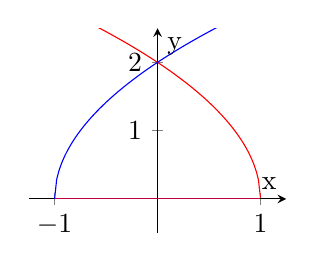
\begin{tikzpicture}
            \begin{axis}[width=0.4\textwidth, axis lines=middle, xlabel=x, ylabel=y, xmin=-1.25, ymin=-.5, ymax=2.5, xmax=1.25, samples=100]
                \addplot[color=green] table[row sep = crcr]{0 0 \\ 1 0 \\};
                \addplot[color=purple] table[row sep = crcr]{-1 0 \\ 1 0 \\};
                \addplot[color=red, domain=-1:1]{2*(1-x)^(1/2)};
                \addplot[color=blue, domain=-1:1]{2*(x+1)^(1/2)};
            \end{axis}
        \end{tikzpicture}
    \end{figure}
\end{example}
\subsubsection{Change of Variables in Multiple Integrals}
To see how a change of variables affects a double integral, first consider a transformation $T: (u,v) \mapsto (x,y)$ whose domain includes a rectangle $S$ in the $uv$ plane with a lower left corner at $(u_0, v_0)$ and an upper right corner at $(u_0 + \Delta u, v_0 + \Delta v)$. \par
The image of $S$ is a region $R$ in the $xy$ plane with one boundary point at $(x_0, y_0) = T(u_0, v_0)$ and another at $\vec x_1 = T(\vec u_1)$. The vector $T(u, v) = \vec r(u, v) = \<x(u, v), y(u,v)\>$ is the position vector of the image of the point $\vec u$. \par
We can obtain functions for the images of each of the edges of $S$ that stem from the lower left corner by fixing one of either $u$ or $v$ at $(u_0, v_0)$ and allowing the other to vary from the up to $(u_0+\Delta u, v_0 + \Delta v)$. This gives us
\[ \vec r_u = \vec r (u, v_0), \quad u\in[u_0, u_0+\Delta u] \]
\[ \vec r_v = \vec r (u_0, v), \quad v\in[v_0, v_0+\Delta v] \]
Then, the tangent vector to each of these image curves is given by
\[ \vec T_u = \< x_u(u_0, v_0), y_u(u_0, v_0)\> \]
\[ \vec T_v = \< x_v(u_0, v_0), y_v(u_0, v_0)\> \]
We can then approximate the image of $S$ under $T$ as a parallelogram with its left side given by the difference vector $\vec r(u_0, v_0 + \Delta v) - \vec r(u_0, v_0)$ and the bottom side given by $\vec r(u_0 + \Delta u, v_0) - \vec r(u_0, v_0)$. \par
If you look closely at these vectors, they look quite similar to the definition of the partial derivative. That is,
\[ \vec T_u = \lim_{\Delta u\to 0}\frac{\vec r(u_0 + \Delta u, v_0) - \vec r(u_0, v_0)}{\Delta u} \]
and 
\[ \vec T_v = \lim_{\Delta v\to 0}\frac{\vec r(u_0, v_0 + \Delta v) - \vec r(u_0, v_0)}{\Delta v} \]
From this, we can say
\[ \vec r(u_0 + \Delta u, v_0) - \vec r(u_0, v_0) \approx \Delta u \vec T_u \]
\[ \vec r(u_0, v_0 + \Delta v) - \vec r(u_0, v_0) \approx \Delta v\vec T_v \]
The area of $T(S)$ is approximately equal to the area of the parallelogram with sides approximately given by $\Delta u \vec T_u$ and $\Delta v \vec T_v$. The area of this can be computed using the cross product
\[ \Delta A = \norm{\Delta u \vec T_u \times \Delta v \vec T_v} = \norm{\vec T_u \times \vec T_v}\Delta u\Delta v\]
Computing the cross product,
\begin{align*}
    \norm{\vec T_u \times \vec T_v} &= \norm{\begin{vmatrix}
        \ihat & \jhat & \khat \\
        x_u(u_0, v_0) & y_u(u_0, v_0) & 0 \\
        x_v(u_0, v_0) & y_v(u_0, v_0) & 0
    \end{vmatrix}} \\
    &= \begin{vmatrix}
        x_u(u_0, v_0) & y_u(u_0, v_0) \\
        x_v(u_0, v_0) & y_v(u_0, v_0)
    \end{vmatrix} \\
\end{align*}
The determinant that arises in this calculation is known as the \it{Jacobian} of $T$ and is given a special notation.
\begin{definition}
    The \bf{Jacobian} of a transformation $T$ given by $x = x(u, v)$ and $y = y(u, v)$ is
    \[ \frac{\partial(x,y)}{\partial(u,v)} = \begin{vmatrix}
        \pdv{x}{u} & \pdv{x}{v} \\
        \pdv{y}{u} & \pdv{y}{v}
    \end{vmatrix}\]
\end{definition}
With this notation, we can writ a concise approximation of $\Delta A$:
\[ \Delta A \approx \abs{\pdv{(x,y)}{(u,v)}}\Delta u\Delta v\]
Where the Jacobian is evaluated at $(u_0, v_0)$. \par If we divide a region $S$ in the $uv$ plane into rectancles $S_{ij}$ and call their images in the $xy$-plane $R_{ij}$, we can apply the approximation from the Jacobian and find
\begin{align*}
    \iint\limits_R f(x,y)\dd y\dd x &= \lim_{m,n\to\infty}\sum_{i=1}^n\sum_{j=1}^m f(x_i, y_i)\Delta y \Delta x\\
    &=\lim_{m,n\to\infty}\sum_{i=1}^n\sum_{j=1}^m f(x(u_i,v_j), y(u_i,v_j))\abs{\pdv{(x,y)}{(u,v)}}\Delta u\Delta v \\
    &= \iint\limits_D f(x(u,v), y(u,v))\abs{\pdv{(x,y)}{(u,v)}}\dd u\dd v
\end{align*}
\begin{theorem}[Change of Variables in a Multiple Integral]
    Suppose that $T$ is a $C^1$ transformation whose Jacobian is nonzero and that maps a region $S$ in the preimage space $U$ to a region $R$ in the image space $X$. Suppose that $f$ is continuous on $R$ and that $R$ and $S$ can be described with one variable as a function of the others. Suppose also that $T$ is one-to-one, except perhaps on the boundary of $S$. Then,
    \[ \int\limits_R f(x_1, \dots, x_n)\dd ^n \vec x = \int\limits_S f(x_1(u_1, \dots, u_n), \dots, x_n(u_1, \dots, u_n))\abs{\pdv{(x_1, \dots, x_n)}{(u_1, \dots, u_n)}}\dd ^n \vec u\]
\end{theorem}
This theorem states that we can change an integral from the $X$ world to the $U$ world by writing
\[ \dd ^n\vec x = \abs{\pdv{(x_1, \dots, x_n)}{(u_1, \dots, u_n)}}\dd ^n \vec u\]
and changing the bounds appropriately.
\begin{example}
    Use the change of variables described by the transformation $T: (x,y)\mapsto(u,v)$ where $x = u^2-v^2$ and $y = 2uv$ to evaluate the integral $\iint_R y\dd A$. $R$ is the region bounded by the $x$ axis and the curves $x = 1-\frac{1}{4}y^2$ and $x=\frac{1}{4}y^2-1$. \par
    \bf{Solution:} First, notice that $R$ is the image of the square $[0,1]\times[0,1]$ under the transformation $T$, as we previously found in Example \ref{exsquare}. \par
    Now, we can compute the Jacobian for a transformation from the $xy$-plane to the $uv$-plane.
    \[ \pdv{(x,y)}{(u,v)} = \begin{vmatrix}
        \pdv{x}{u} & \pdv{x}{v} \\
        \pdv{y}{u} & \pdv{y}{v}
    \end{vmatrix} = \begin{vmatrix}
        2u & -2v \\
        2v & 2u
    \end{vmatrix} = 4u^2+4v^2 > 0\]
    And plug in.
    \begin{align*}
        \iint\limits_R y\dd A &= \iint\limits_S 2uv\abs{\pdv{(x,y)}{(u,v)}}\dd u \dd v \\
        &= \int_0^1\int_0^1 [8u^3v+8uv^3]\dd u \dd v \\
        &= \int_0^1 [2v + 4v^3]\dd v = 2 
    \end{align*}
\end{example}
% \begin{example}
%     Evaluate the integral $\iint_R e^{(x+y)/(x-y)}\dd A$ where $R$ is the trapezoidal region with vertices $(1,0)$, $(2,0)$, $(0, -2)$, and $(0, -1)$. 
% \end{example}
\begin{example}  
    Find the Jacobian determinant \( \abs{\pdv{(x,y,z)}{(\rho,\phi,\theta)}} \) for transforming between rectangular coordinates and spherical coordinates.
    \begin{align*}
        \pdv{(x,y,z)}{(\rho,\phi,\theta)} &= \begin{vmatrix}
            \pdv{x}{\rho} & \pdv{x}{\phi} & \pdv{x}{\theta} \\
            \pdv{y}{\rho} & \pdv{y}{\phi} & \pdv{y}{\theta} \\
            \pdv{z}{\rho} & \pdv{z}{\phi} & \pdv{z}{\theta}
        \end{vmatrix} = \begin{vmatrix}
            \cos\theta\sin\phi & \rho \cos\theta\cos\phi & -\rho\sin\theta\sin\phi \\
            \sin\theta\sin\phi & \rho\sin\theta\cos\phi & \rho\cos\theta\sin\phi \\
            \cos\phi & -\rho\sin\phi & 0
        \end{vmatrix} \\
        &= \begin{vmatrix}
            \cos\theta\sin\phi & \rho \cos\theta\cos\phi & -\rho\sin\theta\sin\phi \\
            \sin\theta\sin\phi & \rho\sin\theta\cos\phi & \rho\cos\theta\sin\phi \\
            \cos\phi & -\rho\sin\phi & 0
        \end{vmatrix} \\
        &= \cos\phi \begin{vmatrix}
            \rho\cos\theta\cos\phi & -\rho\sin\theta\sin\phi \\
            \rho\sin\theta\cos\phi & \rho\cos\theta\sin\phi
        \end{vmatrix} + \rho\sin\phi\begin{vmatrix}
            \cos\theta\sin\phi & -\rho \sin\theta\sin\phi \\
            \sin\theta\sin\phi & \rho\cos\theta\sin\phi
        \end{vmatrix} \\
        &= \cos\phi\pqty{\rho^2\cos^2\theta\sin\phi\cos\phi + \rho^2\sin^2\theta\sin\phi\cos\phi} + \rho\sin\phi\pqty{\rho\cos^2\theta\sin^2\phi + \rho\sin^2\theta\sin^2\phi} \\
        &=\rho^2\sin\phi\cos^2\phi(\sin^2\theta+\cos^2\theta) + \rho^2\sin^3\phi(\sin^2\theta + \cos^2\theta) \\
        &= \rho^2\sin\phi(\cos^2\phi + \sin^2\phi) = \rho^2\sin\phi \\
        \abs{\pdv{(x,y,z)}{(\rho,\phi,\theta)}} &= \abs{\rho^2\sin\phi} = \rho^2\sin\phi
    \end{align*}
    With the absolute value bars being able to be removed because $\sin\phi>0$ in the domain of $\phi\in[0, \pi]$. 
\end{example}